% %set_parent(‘/Users/mwilli/Documents/Spring_2017/Dissertation_Document/Dissertation_Working_Directory_Draft/Dissertation_Main.Rnw')
% 
% <<chunk_options, echo=FALSE>>=
% # This is where we set basic knitr options.
% opts_chunk$set(echo=TRUE, message=FALSE, warning = FALSE, cache = FALSE, comment="")
% options(width=75) # This sets how wide the R printout can be.
% @
% 
%  <<setup-child, include=FALSE>>=
%  set_parent('/home/sam/Dissertation/Dissertation_Template/Dissertation_Main_Template/Dissertation_Main.Rnw')
% @
% 
% <<load_libraries, echo=FALSE>>=
% library(tidyr)
% library(dplyr)
% library(ggplot2)
% library(lme4)
% library(lsmeans)
% library(car)
% library(pbkrtest)
% library(xtable)
% library(cowplot)
% library(plyr)
% @

\chapter{Automatic Speech Recognition of Ear-Recorded Speech\label{chapter4}}


\section{Introduction}\label{chap4:introduction}

The automatic recognition of human speech by a computer has been a subject of interest spanning decades.  Humans first and foremost communicate their ideas via speech and human language, and teaching computers to be able to take verbal instructions would make interaction with them much easier for a majority of the population, particularly the elderly and disabled.  Since this task has been a subject of much study for over half a century, and is only recently gaining much success, it is important to briefly discuss these successes and the challenges that still remain.
% Despite these successes, challenges still remain when there is noise in the signal (\cite{zhang:17}).   
%As before, it is important to understand the mechanics and acoustics of why this proves to be a challenge for automatic speech recognition (ASR), and traditional methods of dealing with this as well as more modern techniques.

The present study proposes a new technique to be used in the advancement of noise-robust automatic speech recognition (ASR).
The experiment in Chapter \ref{chapter2} collected ear-recorded speech data, which aimed to overcome the difficulty of accurately perceiving speech in a noisy environment, for recognition both by computer (ASR) or by human speech perception.  This data will be used in an experiment utilizing the standard open-source ASR system Kaldi (\cite{povey:11}) with the standard, freely-available acoustic model developed from the LibriSpeech corpus (\cite{panayotov:15}).

% It is important to first understand the mechanics behind automatic speech recognition in order to understand the difficulties posed by noise in the signal. The background will take the form of a high-level walk-though of ASR architecture.  A very basic visualization of how signal processing quantifies speech in noise will be given first, followed by the ASR walk-through. Solutions proposed to address issues arising from speech in noise will be woven into this description.

\section{Background}
\label{chap4:background}

% Things to hit on:
% - Base-level Acoustics-to-Features
% - Traditional general ASR mechanics?
% - Current methods of ASR (Cutajar + more recent)
% - Outline problem of noise in the signal
% - Traditional methods of filtering noise out of the signal
% - Previous methods of ASR in noise
% -- Issues with these traditional methods (of removing noise and ASR in noise)
% - Current methods of ASR in noise (Li 2014, and more current)
% -- Multiple Microphones and Beamforming
% -- Other methods??  Look at current CHiME challenge papers
% - Try to find continued issue with electronically identifying speech in noise
% - Emphasize unpredictability of noise, and unknown amplitude - how ear-recorded speech may be able to `protect' against this unpredicatability

% The basics of the acoustics of speech was discussed at the beginning of Chapter \ref{chapter2}.  As a recap, speech contains voiced and voiceless sounds.  The voiceless sounds are generally produced by turbulence - air moving rapidly through a small openning in the vocal tract.  The voiced sounds are more complex, and contain harmonics (acoustic energy focused in very narrow bands of frequency).  Certain harmonics (out of the full set of harmonics in the voiced signal) contain more energy than the other harmonics; these regions in the frequency spectrum with harmonics containing greater energy are called formants, and this is where much of the speech information comes from.
% 
% The human auditory system does a remarkable job of finding these acoustic features and interpreting them, but a computer does not have an inherent auditory system and (as of now) needs to be told what to look for.  Simply put, via a microphone, computers receive a series of digits (numbers) which correspond to the amount of pressure at a given point in time.  
% %
% \begin{wrapfigure}{L}{0.5\textwidth}
% \centering
% 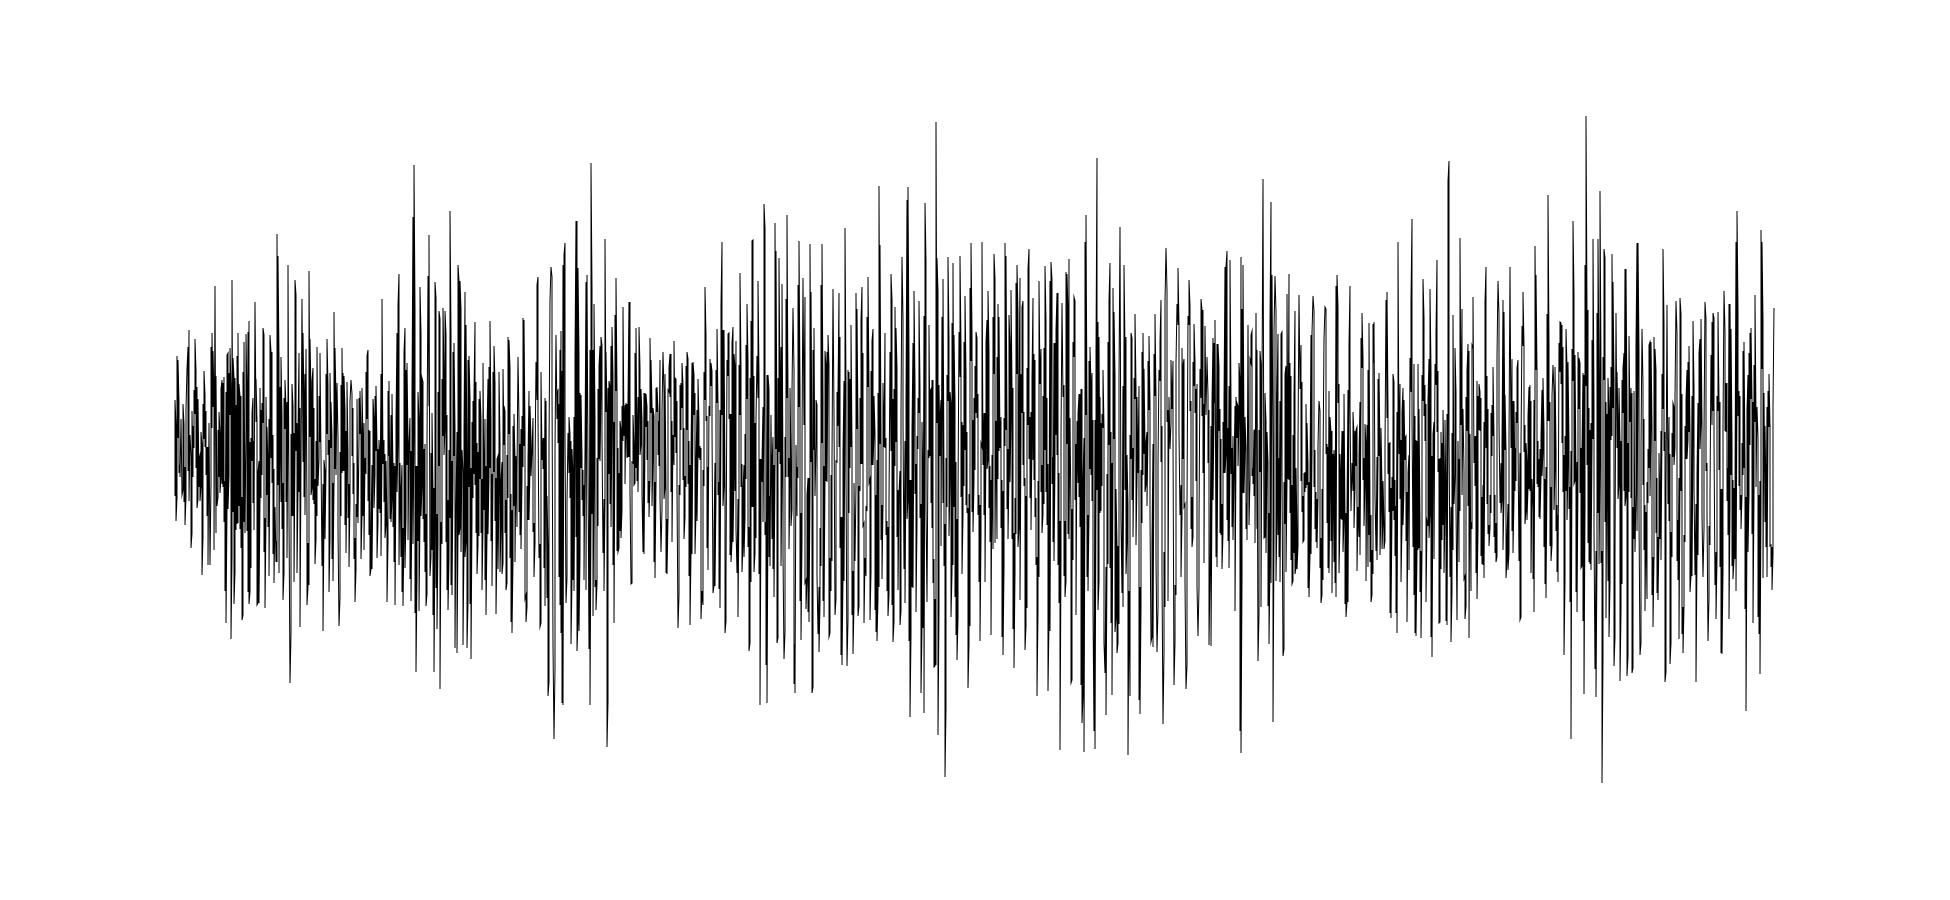
\includegraphics[width=0.45\textwidth]{figure/single-channel-animals.png}
%   \caption{A waveform graph representing the high and low pressure fluctuations that comprise sound.}
%   \label{fig:waveform}
% \end{wrapfigure}

While there are more than 30 years of research involving ASR, and nearly as many working with speech in noisy environments, it is impossible to mention all or even most techniques within this very brief overview.  Therefore, %the discussion will highlight only several `noise-robustness' methods that are used at each level of processing along the ASR pipeline. 
 only several areas of research in noise-robust ASR that pertain to the present study will be discussed.

Equation \ref{eq:basic} is often used to represent the combination of speech and noise,
\begin{equation}\label{eq:basic}
y = x \cdot h + n
\end{equation}
where $x$ is the clean speech signal, $h$ is any convolution (eg. room reverberation, microphone channel warp, etc.) of the original speech signal, $n$ is additive noise, and $y$ is the noisy speech signal.  In addition, the phase of the component signals contributing to the resulting signal $y$ also has an effect.  Taking phase into account means that additive noise is not always simply additive, as energy at frequencies with competing phases could cancel each other out to varying degrees, depending on phase (cf. Chapter \ref{chapter1}).  

Generally in speech perception research, phase is ignored as it contains no speech information; it does become important, however, when multiple sound sources begin to interact substantially. While there is some research that does take phase into account and demonstrates that by doing so, more accurate noise removal can be achieved (eg. \cite{deng:04,leutnant:09}), attempting to model phase adds significant complexity, and the problematic (many researchers admit) assumption is frequently made in ASR that phase plays no role and is consequently ignored (\cite{li:14}).  

% \section{Mechanics of ASR}
% 
% \subsection{The Incoming wave}
% 
% For illustration, the word $W$ is spoken and sent to an ASR recognizer.  This, acoustically in the temporal domain, takes the form seen in the waveform graph if Figure \ref{fig1}.
% 
% \begin{figure}[h!]
% INSERT WORD WAVEFORM - fig1
% \end{figure}
% 
% When encoded digitally for the ASR system, it takes the form of a series of numbers, each number corresponding to normalized pressure value along the waveform (cf. Fig. \ref{fig2}).  These occur in a vectorized format (cf. Fig. \ref{fig3}).  `Sample' is the term that will be used to referred to an individual numeric value in the `sample vector' seen in Figure \ref{fig3}.  Therefore, the `sample rate' is the number of samples in a given length of time (generally normalized to 1 second).  For example, for ASR research, a common sample rate is 16 kHz, ie. 16,000 samples are used to represent a 1-second portion of a waveform.
% 
% \begin{figure}[h!](A)(B)
% INSERT Waveform w/ number points - fig2
% \end{figure}
% 
% \begin{figure}[h!](A)(B)
% INSERT vector w/ numbers (same numbers as in plot above) - fig3
% \end{figure}
% 
% A prespecified `window' size will divide the sample vector into `chunks', or `windows'.  Typically, this window is given in terms of milliseconds, since the number of samples in a specified length of time varies depending on the sample rate.  Typical window sizes range in width from \textbf{X} to \textbf{Y} milliseconds.  The first window will start at the first sample of the speech signal.


%%%%%%%%%%%%%%%%%%%%%%%%%%%%%%  OLD LIT REVIEW  %%%%%%%%%%%%%%%%%%%%%%%%%%%%%%%%%
%Multi-style training, what it is (training with multiple types of noise) - it is ineffective.  Older - paper cited was written in 1987. \cite{li:14}, \cite{lippmann:87}.

%The categorization of noise-robustness techniques utilized by hundreds of researchers over the years is difficult, but, broadly, two domains can be outlined (\cite{li:14,zhang:17}).  
ASR architecture can be categorized into two primary domains. The first is the `feature-space' domain, which focuses on front-end processing of the signal $y$ itself.  The second group utilizes the `model-space' domain, or the back-end processing that contains probability distributions and makes predictions about a signal. %modifies the acoustic model to account for any noise in the signal $y$.    
Noise can be accounted for in either the feature space domain or the model space domain, or occationally, both.  %In the feature domain, noise is dealt with, and the signal is enhanced, prior to sending the features to the acoustic model for recognition.  These modifications are made without altering the acoustic model parameters, resulting in low computation cost.  In the model space, acoustic parameters themselves can be modified in accordance with the noisy signal.  This generally results in high computation cost when training the acoustic model.  There is normally a trade-off between the two domains: one of computation efficiency and performance. Model space alterations often yielding higher performance improvement, while feature space alterations are less computationally intensive (\cite{li:14}).
%Advances in neural network technology have also lent itself to application in noise-robust ASR.  These have provided additional methods of tackling the problem.

\subsection{Feature Space Domain}

Feature space is the part of the ASR process where an acoustic signal is transformed into `features' describing salient parts the acoustic signal that the ASR model will receive as input. The typical features used in ASR applications are Mel-Frequency Cepstral Coefficients (MFCCs) and Perceptual Linear Prediction (PLP) coefficients. The process to calculate these features involves a number of steps, which is described below.  In the feature domain, noise is dealt with, and the signal is enhanced, during or directly after feature extraction and prior to sending the features to the acoustic model for recognition.  These methods are introduced after feature extraction via MFCC or PLP calculation is described.

\subsection{MFCC Calculation}\label{sec:mfcc-calc}

First, a very brief window of the acoustic signal is taken; this is typically 25 milliseconds in length, but can range from 20-40 ms (\cite{vergin:99,molau:01}); each windowed portion of the signal is called a frame.  The frame is then passed through some variety of a Fourier Transform (most often a Fast Fourier Transform, ie. FFT) that converts the signal into its spectral components in the frequency domain.  The power spectrum, sometimes referred to as the energy spectrum, is calculated from the frequency spectrum by\footnote{Equations in this section are derived from \cite{vergin:99}}: \begin{equation}\label{eq:power-spectrum} P_k = |S(k)|^2 \end{equation} where $S$ is the frequency spectrum, $k$ is the frequency component, and $P$ is the power spectrum.

A series of Mel-frequency filters are then applied to the power spectrum.  The frequency spectrum is generally shown with a linear scale, the linear unit of measurement being Hertz.  This (Hertz) is the absolute measure of the number of repetitions of a component wave per second.  The Mel-frequency scale, by contrast, is logarithmically based.  This means low frequency information is represented in greater detail (ie. narrower-bandwidth filters are used on the lower frequencies), while the higher frequencies are represented in less detail (ie. wider-bandwidth filters are used).  One purpose of a logarithmic scale is to better model the human auditory system, which perceives frequencies in a logarithmic basis, ie. humans perceive the lower frequency range in more detail than the higher frequency ranges (\cite{rosen:91}).

The Mel-frequency filterbanks, consequently, are heavily concentrated in the lower [linear] frequencies (cf. Fig. \ref{fig:filt-mfcc}) due to the logarithmic nature of the scale, and are spread out in the higher frequencies. The filters themselves take the shape of a triangle.  The number of filter banks applied to the power spectrum can vary from 20-40 (\cite{honig:05,gold:11}) depending on the methodology. 

\begin{figure}[h]
\centering
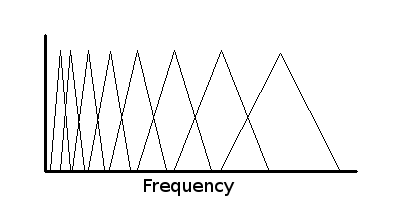
\includegraphics[width=0.75\textwidth]{figure/filt-mfcc.png}
\caption{Demonstration of triangular Mel-frequency logarithmic filters. Scale is not exact.}\label{fig:filt-mfcc}
\end{figure}

Afterwards, the log of each filter output is taken, and a discrete cosine transform (DCT) is applied: \begin{equation}\label{eq:mfcc-calculation} c_m = \beta_c \sum_{j=1}^{J-1} \cos(m\dfrac{\pi}{J} (j+0.5)) \log_{10} (P_j) \end{equation} where $J$ is the number of Mel filterbanks used, $P_j$ power spectrum of filter band $j$, and $m=[1,2,3...,M]$ is the number of cepstral coefficients $c$.  $\beta_c$ is an amplification factor.  Generally for ASR, only the first 12 cepstral coefficients are used, ie. $M=12$; this also has the effect of `smoothing' the cepstral representation of the spectrum, reducing the effect of noise (\cite{gold:11}).  These 12 cepstral coefficients comprise the MFCC vector $c$.  While sometimes these 12 MFCC components compose the acoustic vector alone, it is also standard to add the frame's `energy' component to the end of this vector.  This vector contains the 13 `raw' feature components of the acoustic feature vector (\cite{jurafsky:09}).  

The frame is then shifted temporally, generally by 10 ms, to obtain the next frame. This temporal shift is called the `step', and the duration of the shift (eg. 10ms) is called the `step size'.  The acoustic vector is then calculated for this - and subsequent - frames in the speech signal.

While the traditional acoustic vector captures speech information from a single frame, or acoustic window, it is also useful to explicitly model how these features change from frame to frame.  An additional set of 13 features\footnote{The standard 13 features will be assumed, but this can be a vector of length 12 if `energy' is not used.} can be calculated by\footnote{Delta and Delta-Delta equations are derived from \cite{gold:11}.} \begin{equation} d_t = \dfrac{\sum_{n=1}^{N} n(c_{t+n} - c_{t+n})}{2\sum_{n=1}^{N} n^2} \end{equation} where $c_t$ is the acoustic vector at time $t$, $n$ is the number of acoustic vectors in either direction (from $t$) that will be included in the calculation (generally, N=2), and $d_t$ is the delta vector at time $t$.  

If delta vectors encode the change in cepstral and energy values, delta-delta vectors encode the change in delta vectors.  These are computed in the same way, though delta vectors replace the cepstral vectors in the calculation, such that \begin{equation} dd_t = \dfrac{\sum_{n=1}^{N} n(d_{t+n} - d_{t+n})}{2\sum_{n=1}^{N} n^2} \end{equation} where $dd_t$ is the delta-delta vector at time $t$.  Both delta and delta-delta vectors have the same length as the cepstral vector, 13, so that when combined, they yield an acoustic feature vector with 39 features.  %This calculation hierarchy can be visualized in Figure \ref{fig:mfcc-hier}.  
Delta and delta-delta computation is quite standard procedure for modern ASR systems (\cite{htk:15}).


\subsection{Perceptual Linear Prediction}\label{sec:plp}

An alternative to MFCC feature vectors that generally results in more noise-robust features is perceptual linear predictive cepstral coefficients (PLP; \cite{hermansky:85}).  The first few steps in PLP calculation are the same as in MFCC calculation.  A window is used to extract a frame of audio (generally between 20-40 ms), a FFT is computed and the power spectrum (cf. Equation \ref{eq:power-spectrum}) is computed from that.  PLP obtains its `perceptual' moniker by implementing the following: critical band filtering, `equal-loudness' pre-emphasis, and the conversion from intensity to loudness.  

Unlike the triangular filters used in the Mel-filtering for MFCC calculation, PLP makes use of `critical band' filters (cf. Fig \ref{fig:filt-cb}).  These trapezoidal filters are intended to incorporate an implementation of critical bands as they are observed in the cochlea. Physiologically, these `critical bands' are regions in the cochlea (along the basilar membrane) which respond to, or are activated by, a range of frequencies (\cite{fletcher:40}).  These critical bands are logarithmic in that the critical bandwidth of lower-frequency regions is narrower (ie. higher resolution of lower frequencies) and is wider in higher-frequency receptor regions of the cochlea.  In application, the trapezoidal `critical band' filters used for PLP utilize the Bark-frequency scale (also logarithmic, similar to the Mel-frequency scale).

\begin{figure}[h]
\centering
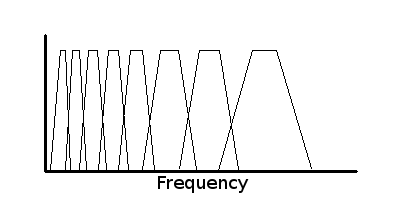
\includegraphics[width=0.75\textwidth]{figure/filt-cb.png}
\caption{Demonstration of trapezoidal critical band logarithmic filters. Scale is not exact.}\label{fig:filt-cb}
\end{figure}

After the critical band filterbank is constructed, `equal-loudness' pre-emphasis is applied.  This is very similar to conventional preemphsis (increasing the amplitude of higher frequencies), but follows the human perceptual frequency-dependent sensitivity of loudness in that it does not emphasize the very high frequencies as much as the mid-range frequencies.% (cf. Fig. \ref{?}, adapted from \cite{honig:05}).  
The explicit conversion from intensity to loudness is then performed on these preemphasized, critical band filterbanks by effectively compressing the signal by taking the cubic root of the values in the filterbanks.

Following these perceptually-based transforms, an inverse Discrete Fourier Transform is performed to return the signal to the time domain (from the power domain), and a linear predictive (LP) filter (such as the Levinson Durbin algorithm) is applied to the time-domain signal (\cite{gold:11}).  This has the effect of smoothing out the variance in the spectral envelope (if it were to be reconverted to the spectral domain).  During this process, autoregressive weights (coefficients) are trained on the time-domain signal which are used in the LP filter.  Using a recursive formula these LP coefficients are converted into cepstral coefficients - the same unit used in MFCCs.  It is the LP component, and the smoothing of the signal and hence the spectral envelope, that produces much of the specific benefit given to PLP when recognizing speech in noise.  While the perceptual-based transformations offer recognition benefit, some have found that Mel-frequency filter banks can perform as well or better than Bark-frequency critical band filterbanks (cf. \cite{honig:05}).

MFCC and PLP are the two primary methods used to extract cepstral coefficients that are most widely used in ASR architecture.  On top of these `feature-generation' pipelines, many methods have been proposed to further remove ambient noise from the features.

\subsection{RASTA and CMVN}\label{sec:rasta_cmvn}

RASTA (RelAtive SpecTrAl methodology) is a noise-robust technique designed specifically to fit into the PLP feature extraction algorithm (\cite{hermansky:92}).  After the critical band filterbank is applied in PLP processing, the logarithm of these values is obtained.  In log-space, a bandpass filter transfer function is traditionally applied, but a number of other filtering techniques could be used here.  Equal-loudness pre-emphasis and intensity-to-loudness conversion are also performed in log-space, before the exponent (reverse-log) is taken, and PLP calculation resumes as normal.

The reason for the utilization of log-space is to take advantage of its special properties in order to remove (primarily) convolutional noise (\cite{gold:11}).  Recall Equation \ref{eq:basic}, where $x$ is the source signal, $h$ is a convolutional noise, and $y$ is the resulting `noisy' signal at time $t$.  In the spectral domain, this transforms into \begin{equation} Y(f) = X(f)H(f) \end{equation} where $Y$, $X$ and $H$ are the spectral representations of $y$, $x$, and $h$ with frequency bin $f$, and the relationship between $X$ and $H$ is multiplicative.  Therefore, the conversion to the log domain yields \begin{equation} \log(Y(f)) = \log(X(f)) + \log(H(f)) \end{equation} where the relationship between $X$ and $H$ now becomes additive, and consequently much easier to account for.  The RASTA technique is most useful when signal distortion is caused by some sort of convolution, or by some sort of steady-state noise.

Another common procedure, similar to RASTA in that it primarily removes signal distortion or steady-state noise, is Cepstral Mean Normalization, or Cepstral Mean and Variance Normalization (CMN and CMVN;\cite{atal:74,viikki:98}).  To calculate the cepstral mean and variance, a window of cepstral feature vectors is required.  Because of this, there will be a brief delay of $N$ multiplied by the frame window shift in milliseconds, where $N$ is the number of frames to incorporate into the mean and variance calculations.  If $N=20$, which is the minimal acceptable value given by \cite{viikki:98} and the step size is a standard 10ms, then the delay in calculating each cepstral value would be 200ms.

The mean is calculated by\footnote{Equations adapted from \cite{viikki:98}} \begin{equation} m_t(i) = \dfrac{1}{N}\sum_{t=1}^{N} c_t(i) \end{equation} where $c_t$ is the cepstral vector at time $t$, $i$ is the $i^{th}$ cepstral coefficient feature in the vector, and $m_t$ is the rolling mean at time $t$.  The N frames that follow $c_t$ are used to calculate the mean cepstral vector $m_t$.  The variance is calculated \begin{equation} \sigma_t(i) = \sqrt{\dfrac{1}{N}\sum_{t=1}^{N} [c_t^2(i)] - [m_t(i)]^2} \end{equation} where $\sigma_t(i)$ is the cepstral variance used for the cepstral coefficient $i$ at time $t$.  The new cepstral value is \begin{equation} \hat{c}_{t-N}(i) =  \dfrac{c_{t-N}(i) - m_t(i)}{\sigma_{t}(i)} \end{equation} where the mean is subtracted by the cepstral value, and then normalized by the variance.  Note $t-N$, because the recalculated cepstral value at time $t$ uses the mean and variance computed at $t+N$.

The frame delay $N$ prevents real time recognition, as it can become rather large, even as long as the whole utterance (\cite{li:14}).  Nevertheless, CMVN is a simple calculation which can result in significant improvement of convoluted signals, or signals with steady state noise, such as an environment with a noisy car (\cite{viikki:98}).

\subsection{Spectral Subtraction and Wiener Filtering}\label{sec:spec-sub_wiener}

Spectral subtraction (\cite{boll:79} is an intuitive method of removing noise by taking a frame, converting the signal into the spectral domain, and subtracting an estimated noisy signal. Simply, ignoring convolution, if linearly \begin{equation} y(t) \approx x(t) + n(t) \end{equation} (cf. equation \ref{eq:basic}) and spectrally \begin{equation} Y(f) \approx X(f) + N(f) \end{equation}, then \begin{equation} \hat{X}(f) \approx Y(f) - \hat{N}(f) \end{equation}.  On a practical level, the power spectra (equation \ref{eq:power-spectrum}) are used in calculations.  $N(f)$ is estimated by computing the mean power spectrum $\mu(f)$ of noise during non-speech portions of the signal.  This results in \begin{equation} |\hat{X}(f)|^2 \approx |Y(f)|^2 - \mu(f) \end{equation} where the power spectrum of $X(f)$ is estimated from the noisy power spectrum $Y(f)$ minus the mean of the power spectra $\mu(f)$ calculated during the portion of the signal preceding speech. $X(f)$ can either be converted back into the time domain, or the power spectra could be used for calculation of MFCC or PLP coefficients.  The process is repeated all along the waveform.

This method still has several problems (\cite{li:14}). First and foremost, the location of speech in the signal in a noisy environment is difficult to detect.  The accurate estimation of the mean of the noise power spectra $\mu(f)$ depends on the ability to accurately detect the onset of speech and to stop the calculation of the average.  Spectral subtraction also requires relatively stationary, slow-variation noise; the use of the mean noise spectra $\mu(f)$ critically assumes that the noise during the speech signal $x$ has an approximate power spectra of $\mu(f)$.  Furthermore, this is only an average of the noise, and not exactly the noise itself.  This subtraction of $\mu(f)$ can inadvertently have an additive noise effect by producing extraneous acoustic artifacts in the `clean' signal which were not there to begin with (\cite{berouti:79}).

Wiener filtering (\cite{lim:79}) is another method used to remove noise from a signal, and is, theoretically, a specific kind of spectral subtraction (\cite{agarwal:99}), though there are some differences. The Wiener filter is calculated in the frequency domain, but unlike Spectral subtraction, can be applied in either the frequency or time domain. There are many modifications to the Wiener filter, one in particular, the two-stage Mel-warped Wiener filter used in the Advanced Front End algorithm (cf. Section \ref{sec:background-afe}) is applied in the time domain.
However, just as with spectral subtraction, Wiener filtering requires an estimate of the noise $|N(f)|^2$ in the the signal.  Furthermore, it does not do well in very low SNR environments, as it generally results in suppression and dampening of the entire signal, and not just the noise (\cite{li:14}).


\subsection{The Advanced Front End Standard}\label{sec:background-afe}

The Advanced Front End (AFE) is a standard noise-reduction algorithm established in 2002 by the European Telecommunications Standards Institute (ETSI; \cite{etsi:02}).  It is comprised of three different algorithms: two-stage Mel-warped Wiener filtering (\cite{agarwal:99}), SNR-dependent Waveform Processing (\cite{macho:01}), and blind equalization (\cite{mauuary:98}).  It yields more than 50\% improvement over standard MFCC features alone, and has become a frequent baseline for comparison in noisy ASR research.

Two-stage Mel-warped Wiener filtering is an adapted form of the Wiener filter that, obviously, Mel-warps the filter, and utilizes two applications of the filter onto the noisy signal $y$ (\cite{etsi:02}).  The process first involves calculating an estimate of the SNR\footnote{Equations in this section are adapted from \cite{etsi:02}} \begin{equation}\label{eq:afe:mwwf:snr} SNR(f) = \dfrac{E|S(f)|^2}{E|N(f)|^2} \end{equation} where $E$ indicates an estimate of the speech power spectrum $|S(f)|^2$ or the noise power spectrum $|N(f)|^2$.  Since no actual filtering is done at this point, the speech power spectrum is first estimated, a variation of spectral subtraction (ie. $|Y(f)|^2 - E|N(f)|^2$, roughly).  The Wiener filter $H$ is then calculated by \begin{equation}\label{eq:afe:mwwf:wf} H(f) = \dfrac{\sqrt{SNR(k)}}{1+\sqrt{SNR(k)}} \end{equation}  A new [more accurate] estimation of the speech power spectrum is obtained by multiplying the filter $H(f)$ by the noisy signal $|Y(f)|^2$.  This new estimate $E_2|S(f)|^2$ is then used in equation \ref{eq:afe:mwwf:snr} to obtain a new SNR, to be used in equation \ref{eq:afe:mwwf:wf} which produces a modified Wiener Filter $H_2(f)$.  Most of the heavy work of the AFE ensemble is performed by this Mel-warped Wiener filtering (\cite{li:14}).

This Wiener filter is then Mel-warped, which modifies the frequency spectrum of the filter $H_2(f)$, so Wiener Filter coefficients are now applied to frequencies on a Mel-scale, now notated $H_{mel}(m)$.  A Mel-Inverse Discrete Fourier Transform is then performed to transform the Mel-frequency domain filter into the time domain, \begin{equation} h_{mel}(m_1) = \sum_{m_2=1}^{M} H_{mel}(m_2) x IDCT_{mel}(m_2,m_1) \end{equation} where $M$ is equal to the number of mel-frequency coefficients $m$ in $H_{mel}(m)$, and $IDCT_{mel}$ is a special Inverse Discrete Cosine Transform function, provided in more detail in \cite{etsi:02}.  The time domain Wiener Filter $h_{mel}(m)$ is weighted with a Hanning Window at each Mel-frequency bin $m$, and is then applied to the noisy signal \begin{equation} \hat{s}(t) = \sum_{m=-(M-1)/2}^{(M-1)/2} h_{mel}(m+(M-1)/2) x y(t-m) \end{equation} where $y(t)$ is the noisy signal sample - and $\hat{s}(t)$ the estimated speech sample - at time $t$.  This is iterated throughout all the samples $t$ out of $T=80$ samples in a given 10ms frame for a 8.0 kHz sampled acoustic signal.  This is repeated for all frames in a signal, recalculating the Wiener Filter $H(f)$ from the noisy signal power spectrum estimate $E|N(f)|^2$ and the new speech power spectrum estimate $E|S(f)|$ for each frame.  This filtering is done prior to any feature extraction.

The SNR-dependent Waveform Processing is a methodology used to dampen the low-SNR portions of the waveform, and enhance the high-SNR portions of the waveform (\cite{macho:01}), and is performed after Two-stage Mel-warped Wiener filtering on the temporal waveform.  Voiced speech consists of repetitive glottal pulses, which can be seen in Figure \ref{fig:glot-spect} as dark vertical striations or Figure \ref{fig:glot-wav}.


First, an energy contour based off of the Teager energy contour (\cite{teager:80}) is calculated for all samples $n$ in a $N=200$-sample frame, \begin{equation} E_{cont}(n) = |\hat{s}(n)^2 - \hat{s}(n-1) \cdot \hat{s}(n+1)| \end{equation} where $\hat{s}$ is the output of the Two-stage Mel-warped Wiener Filter.  This contour is then smoothed.  The maxima peaks of the smoothed energy contour $E_{cont}$ are identified by first locating the global maximum in the frame, and then the maxima on either side of the identified global maximum, resulting in $N_{max}$ maxima, where $pos_{max}(n_{max})$ is the sample index in the maxima. A weighting vector $w(n)$ of length $N=200$ (a weight for each individual sample) is created.  For each sample $n$ in $w(n)$, if $n$ falls between \begin{equation}\label{eq:afe:swp:window} \langle [pos_{max}(n_{max})-4], [0.8 \cdot pos_{max}(n_{max}+1)-pos_{max}(n_{max})] \rangle \end{equation}, $w(n) = 1.2$, otherwise $w(n) = 0.8$. That is to say, that the high-SNR portions of the waveform (ie. those beginning 4 samples before a maximum, extending 80\% of the distance to the next maximum; cf. equation \ref{eq:afe:swp:window}) are enhanced by weight value of 1.2, otherwise dampened by a weight value of 0.8.  This manages to enhance the portions of the signal with high SNR, and dampens those with a low SNR.

\begin{figure}[H!]
\centering
\begin{subfigure}{0.75\textwidth}
\centering
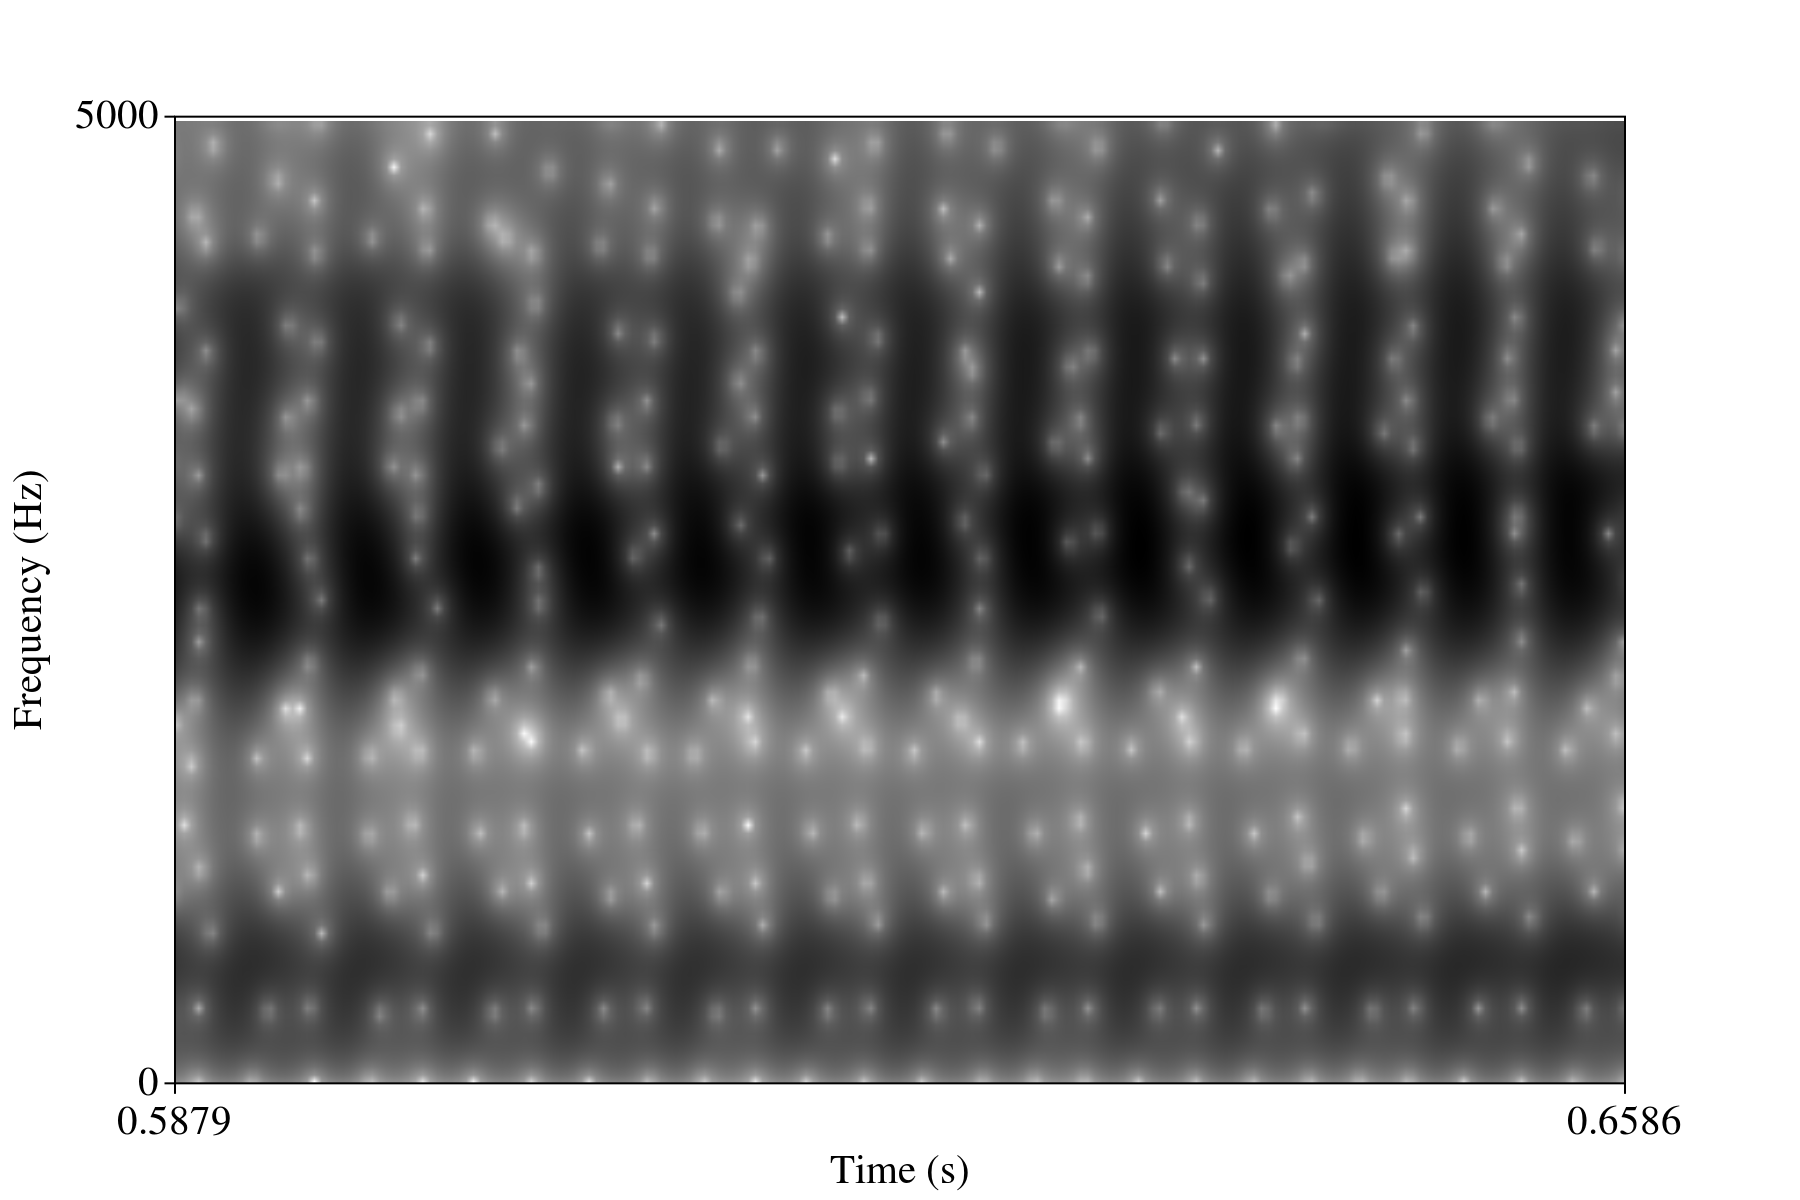
\includegraphics[width=0.65\textwidth]{figure/glot-spect.png}
\caption{A wide-band spectrogram of a portion of /a/. Dark verticial striations (louder amplitude) indicate a periodic glottal pulse}\label{fig:glot-spect}
\end{subfigure}
\begin{subfigure}{0.75\textwidth}
\centering
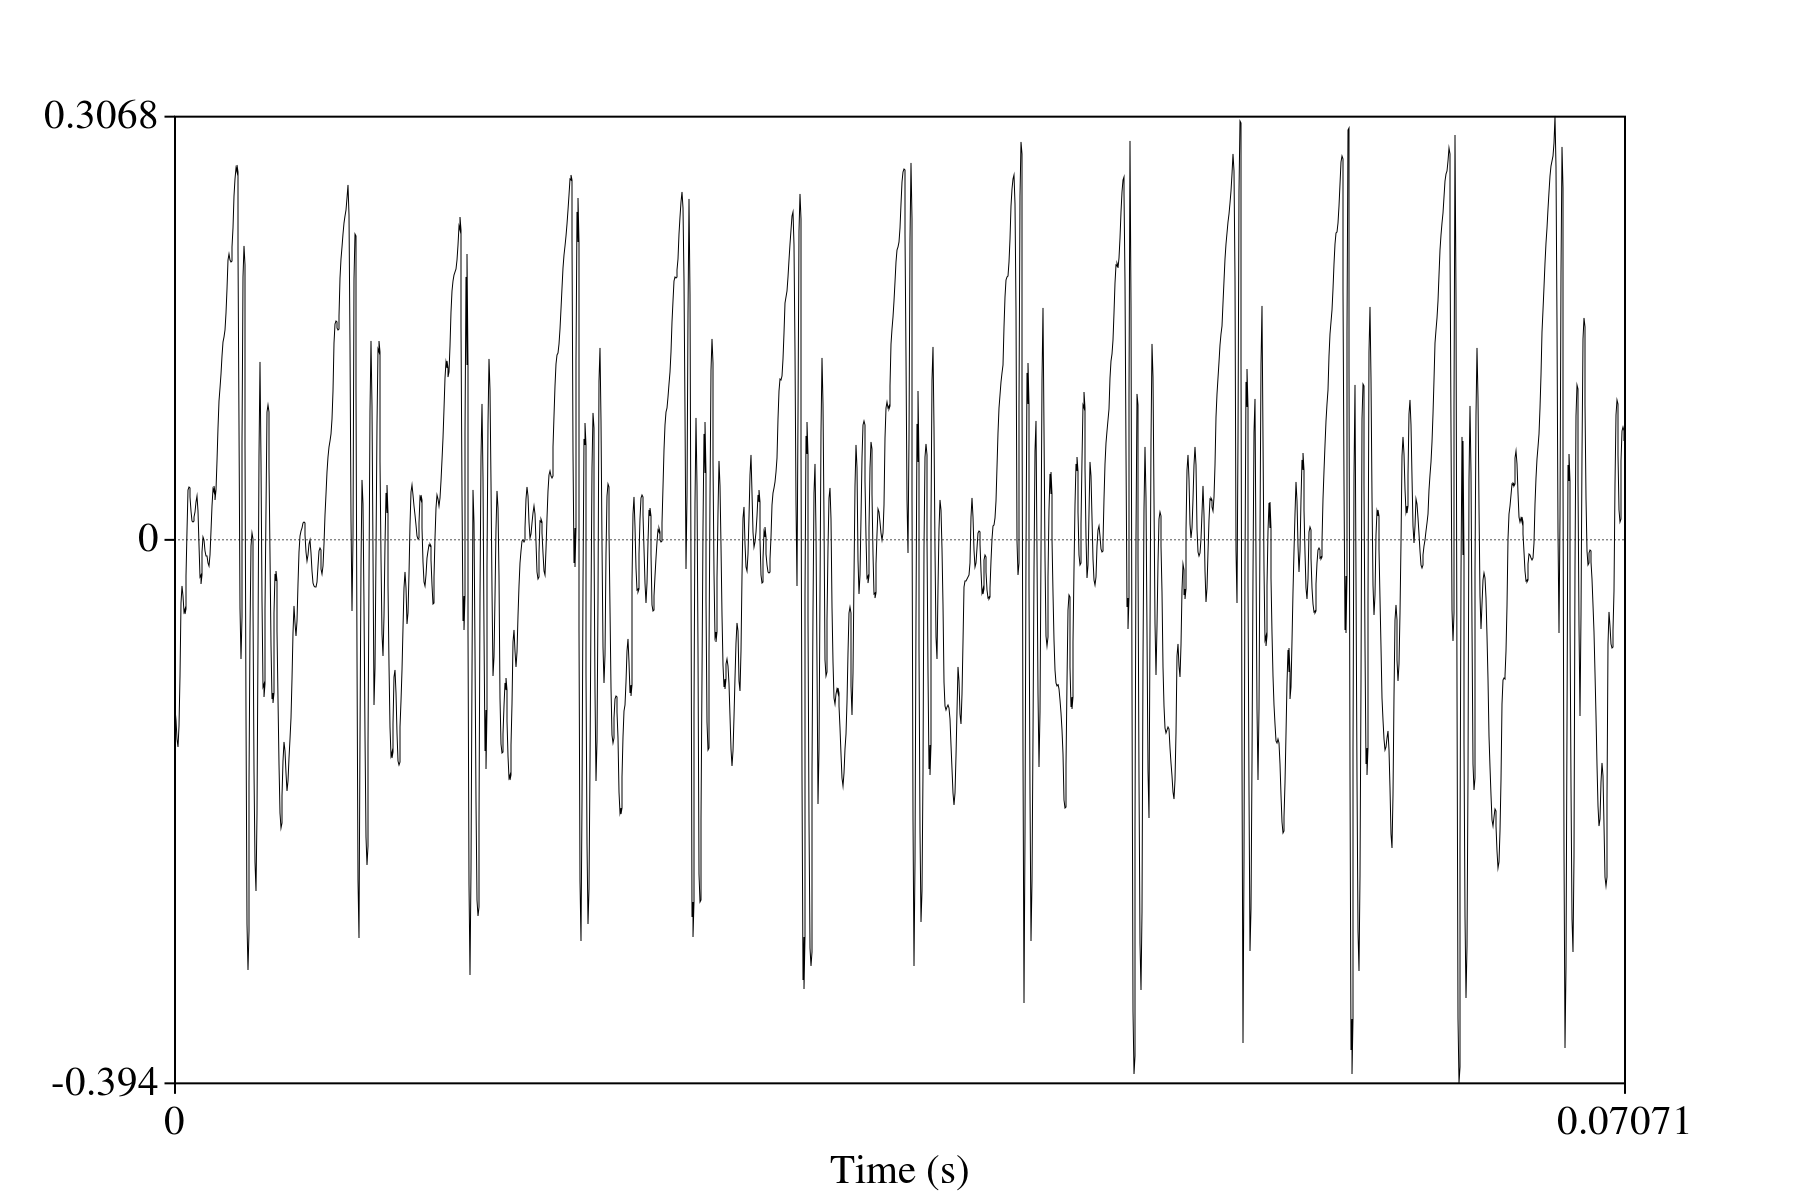
\includegraphics[width=0.65\textwidth]{figure/glot-wav.png}
\caption{A waveform of a portion of /a/.  Periodic peaks are the temporal location of the glottal pulse.}\label{fig:glot-wav}
\end{subfigure}
\caption{Spectrogram and waveform demonstrating periodic glottal pulses.}\label{fig:glot-puls}
\end{figure}

In the feature extraction pipeline, at this point, the signal has been modified in the temporal domain.  Traditional AFE at this point computes the MFCC acoustic feature vectors, largely as described above in Section \ref{sec:mfcc-calc}.  Once the raw feature vector for a frame is obtained (ie. not including delta and delta-delta features), Blind Equalization is performed directly on the 12 cepstral coefficients.

Blind Equalization is the compensation for any convolutive channel distortion imposed on the signal due to recording (\cite{mauuary:98}).  This process is rather straightforward, in that it requires the vector of cepstral coefficients $c(m)$, the energy component $c_{energy}$ from the feature vector of the frame, a bias term $\beta$ which is initialized to $0.0$, and a reference vector of cepstral coefficients $c_{ref}(m)$ which contains coefficients for a flat spectrum (\cite{etsi:02}).  The equalized cepstral vector $c_{eq}$ is computed \begin{equation}\label{eq:afe:be:ceq} c_{eq}(m) = c(m) - \beta \end{equation}, where $\beta = 0.0$ when $m = 1$.  A weighting factor is computed \begin{equation} w = min( 1 , max( 0 , ln(c_{energy}) - \dfrac{211}{64} ) ) \end{equation} which is used in the computation of a step size seen in equation \ref{eq:afe:be:step}. \begin{equation}\label{eq:afe:be:step} w_{step} = 0.0087890625 \cdot w \end{equation}  Between each subsequent cepstral coefficient equalization, the bias term needs to be re-estimated as \begin{equation} \beta \mathrel{{+}{=}} w_{step} \cdot c_{eq}(m) - c_{ref}(m) \end{equation} which is then used in the next cepstral equalization calculation for $c_{eq}(m+1)$ in equation \ref{eq:afe:be:ceq}.

As this is the last step in AFE processing, the equalized raw acoustic feature vector can then be used to compute deltas and delta-deltas, and passed on to the back-end portion of an ASR system, the model domain, described in Section \ref{sec:model-domain} below.  There are hundreds of other proposed noise-reduction techniques which are too numerous to describe here; the methods above have been selected to highlight some of the most well-established front-end mechanisms for feature extraction and noise reduction.


\subsection{Model Space Domain}\label{sec:model-domain}

When the speech signal has been converted from an acoustic vector of audio samples into a set of acoustic feature vectors, these vectors are sent to the back-end model domain.  These vectors can either be used for training an acoustic model, or if an existing acoustic model is to be used, they can be used in the \textit{decoding}, or recognition, of the speech the vectors represent.  There are hundreds of different methods used to train acoustic models, but for the present, very brief overview, only the core principles of acoustic model training will be discussed in a simplified manner.  

\subsection{Training an Acoustic Model}\label{sec:acoust-mod}

Acoustic feature vectors are sent from the front-end feature extraction system to the back-end acoustic modelling mechanism.  The ultimate goal of ASR is to correctly identify the words in a speech utterance; put another way, the goal is to find the most likely utterance transcription given a speech signal.  Simplified further, identify the most likely speech sound, or phoneme, given the feature vector passed from the front-end.  Mathematically, this can be notated as \begin{equation} p(ph|c) \end{equation} where $c$ is the cepstral feature vector (with or without deltas and delta-deltas), and $ph$ is an abstract phoneme.  A related and easier question to ask, mathematically, is \begin{equation} p(c|M_{ph}) \end{equation} or, what is the probability of the feature vector $c$ belonging to the distribution of feature vectors defined by a phoneme model $M_{ph}$.  That is, if the phoneme model $M_{ph}$ were to contain a function that defined which features and feature combinations were representative of the phone $ph$, and the degree to which the features were representative, it could output the probability that $c$ is a feature vector representative of phoneme $ph$.

The traditional and still widely used function that comprises the phoneme model $M_{ph}$ is a Gaussian function (\cite{gales:07}).  A Gaussian put simply, is a normal distribution (cf. Fig. \ref{fig:norm-dist}) that contains a mean $\mu$ and a variance $\sigma^2$; $M_{ph}$ can be represented by \begin{equation} \mathcal{N}_{ph}(\mu,\sigma^2) \end{equation}.  The mean, intuitively, specifies the most likely value, or center, of the distribution.  The variance dictates the width of the distribution; a small variance creates a narrow distribution (cf. Fig. \ref{fig:norm-narrow}) with fewer overall values (along the $x$-axis) and is `taller', whereas a larger variance yields a wide distribution with more values and is `shorter' (cf. Fig. \ref{fig:norm-wide}).  Width indicates how many distinct values fall into the distribution, and height indicates how probably a given value is.  Therefore the center value, the mean, is always the most probable.  It is also necessary that the integration all probabilities of all possible feature values of $f$ in this distribution is 1. \begin{equation} \int_{f=0}^\infty p(f) df = 1 \end{equation}  It is these characteristics that makes a `normal' distribution.  
%
\begin{figure}[H!]
\centering
\begin{subfigure}[c!]{0.5\textwidth}
\centering
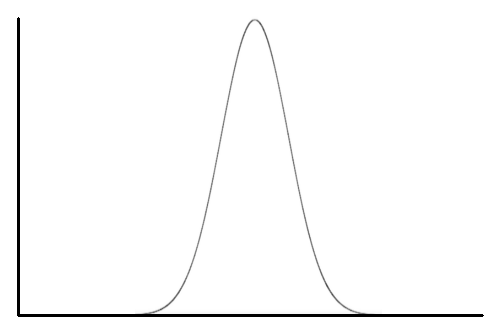
\includegraphics[width=0.5\textwidth]{figure/norm-narrow.png}
\caption{Example of a Gaussian (normal) distribution with a small variance.}\label{fig:norm-narrow}
\end{subfigure}
\qquad
\begin{subfigure}[c!]{0.5\textwidth}
\centering
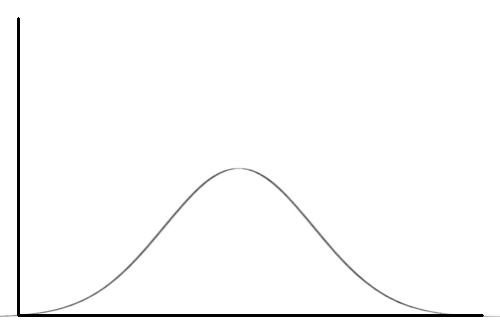
\includegraphics[width=0.5\textwidth]{figure/norm-wide.png}
\caption{Example of a Gaussian (normal) distribution with a large variance.}\label{fig:norm-wide}
\end{subfigure}
\caption{Two Gaussian (normal) distributions with differing variance.}\label{fig:norm-dist}
\end{figure}


This example has shown a one-dimensional Gaussian function.  In reality the Gaussian model of an acoustic feature vector $c$ with length $N$ has $N$ dimensions; if there are 39 features in a vector, one of the 39 dimensions of the Gaussian represents one feature, another dimension represents another feature, and so on.  For example, take the feature vector $c_0(m)$ in first row of the matrix of features in Figure \ref{fig:feat-vectors}.  Each row in this simplified example is a feature vector of the phoneme /u/.  Each column holds the values for a particular feature.  The first feature of the first vector $c_0(0)$ is 12.179.  A Gaussian Model $\mathcal{N}_{/u/}(\mu,\sigma^2)$ trained on this feature alone would result in a mean $\mu=12.179$ and variance $\sigma^2\approx 0$, with \begin{equation} p(c_0(0)|\mathcal{N}_{/u/}(\mu,\sigma^2))\approx 1 \end{equation}  As the model is trained on $c_1(0)$ and $c_2(0)$ and subsequent features, variance begins to develop, and the mean $\mu$ and variance $\sigma^2$ are updated accordingly.
%
\begin{figure}[H!]
\begin{center}
\begin{tabular}{|p{1.5cm}|p{1.5cm}|p{1.5cm}|p{1.5cm}|p{1cm}} \hline
    & $c_n(0)$ & $c_n(1)$ & $c_n(3)$ & $\cdots$ \\ \hline
$c_0(m)$ & $12.179$ & $-2.007$ & $0.059$ & $\cdots$ \\ \hline
$c_1(m)$ & $12.010$ & $-2.279$ & $0.060$ & $\cdots$ \\ \hline
$c_2(m)$ & $11.976$ & $-1.766$ & $-0.002$ & $\cdots$ \\ \hline
\vdots & $\vdots$ & $\vdots$ & $\vdots$ & $\vdots$ \\ 
\end{tabular}
\end{center}
\caption{Cepstral feature vectors $c_0$ through $c_N$.}\label{fig:feat-vectors}
\end{figure}

Thus far only a univariate Gaussian, or a one-dimensional Gaussian has been displayed.  The Gaussian model $\mathcal{N}_{ph}(\mu,\sigma^2)$ used to model an acoustic feature vector is multivariate, or multi-dimensional.  This can be visualized in Figure \ref{fig:two-dim-gauss}, which contains two dimensions ($x$-axis and $y$-axis); each axis has its own mean and variance, and the distribution of the multivariate (two-dimensional) Gaussian is represented by the circles around the datapoints.  
\begin{wrapfigure}{l}{0.5\textwidth}
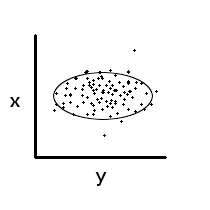
\includegraphics[width=0.5\textwidth]{figure/two-dim-gauss.png}
\caption{Example a distribution along two dimentions, \textbf{x} and \textbf{y}.  The elipse represents the boundaries of the distribution in both \textbf{x} and \textbf{y} dimensions. Distribution is only approximate.}\label{fig:two-dim-gauss}
\end{wrapfigure}
This could also be extended visually into a third dimension, but visualization beyond this breaks down.  It is very difficult to visualize the 39-dimensional Gaussian model $\mathcal{N}_{ph}(\mu,\sigma^2)$ that is used to represent phoneme $ph$; it is essentially a combination of 39 univariate Gaussians into one.
This is [partially] why, for example, a model trained on raw MFCC acoustic vectors (of length 13) cannot recognize feature vectors also including delta and delta-delta features - there is a dimensionality mismatch.


Only single, isolated feature vectors for model training have been used up to this point.  But speech is temporal and context dependent, and it is important to be able to model those characteristics.  For example, a /u/ vowel in the context preceding an /n/ has different qualities than if it were to precede a /t/, due to context dependency.  In ASR, it is normal to take into account the phoneme on either side of the phoneme in question, resulting in a three-phoneme sequence, eg. /t/+/u/+/n/.  These \textit{triphone} sequences use Hidden Markov Models (HMMs) to accomplish this sequence modelling (\cite{jurafsky:09}).

HMMs consist of states $q_i$ and, of transitions $a_{ij}$ between the states.  Each state $q_i$ has an emission probability, $b_i$, the probability of `landing' in state $q_i$. % (cf. Figure \ref{fig:hmm-plain}).  
Each transition has a `transition' probability, $a_{ij}$, ie the probability of transitioning from state $q_i$ to $q_j$.  For ASR, the emission probability of a state is a multivariate Gaussian.  So the state for phoneme /u/ uses the multivariate Gaussian $\mathcal{N}_{/u/}(\mu,\sigma^2)$ to compute its emission probability.  As most ASR systems use triphone acoustic models, the HMMs in these systems have three states in order to model triphones.  An example three-state triphone HMM for the sequence /t/+/u/+/n/ can be seen in Figure \ref{fig:hmm-sounds}.  

\begin{figure}[htbp]
\centering
\tikzstyle{state}=[circle,
                                    thick,
                                    minimum size=1.2cm,
                                    draw=black!80]

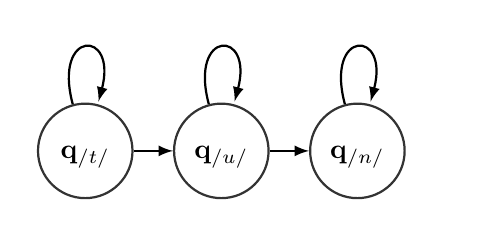
\begin{tikzpicture}[>=latex,text height=1.5ex,text depth=0.25ex]

  \matrix[row sep=0.5cm,column sep=0.5cm] {

        \node (q_{/t/}) [state] {$\mathbf{q}_{/t/}$}; &
        \node (q_{/u/})   [state] {$\mathbf{q}_{/u/}$};     &
        \node (q_{/n/}) [state] {$\mathbf{q}_{/n/}$}; & \\
    };

    \path[->]
        (q_{/t/}) edge[thick] (q_{/u/})	% states via the state
        (q_{/t/}) edge[loop above,thick] (q_{/t/})
        (q_{/u/}) edge[loop above,thick] (q_{/u/})
        (q_{/n/}) edge[loop above,thick] (q_{/n/})
        (q_{/u/})   edge[thick] (q_{/n/})		% accentuated.
        ;

\end{tikzpicture}

\caption{An example HMM with three states, each state representing a different phone.}\label{fig:hmm-sounds}
\end{figure}

The state $q_{/t/}$ has a multivariate Gaussian $\mathcal{N}_{/t/}(\mu,\sigma^2)$ trained to emit its emission probability, as does $q_{/u/}$ have $\mathcal{N}_{/u/}(\mu,\sigma^2)$ and $q_{/n/}$ have $\mathcal{N}_{/n/}(\mu,\sigma^2)$.  In Figure \ref{fig:hmm-sounds}, there are transition probabilities from one state to another (eg. the probability of transitioning from state $q_{/t/}$ to $q_{/u/}$), but also transitions from one state to itself (eg. the probability of transitioning from state $q_{/t/}$ to $q_{/t/}$).  Recall from Section \ref{sec:mfcc-calc} that a normal duration of a frame of audio used for feature extraction is 25ms; ie. each feature vector corresponds to 25ms of audio.  Most phonemes have a duration longer than 25ms, and so there is a need to transition back to itself if the subsequent feature vector indicates that the phoneme has not changed.  The probability for any state $q_i$ to transition to itself is \begin{equation} p(q_i|q_i) = a_{ii}\cdot b_i \end{equation} and the probability to transition to any other state $q_j$ is \begin{equation} p(q_j|q_i) \approx a_{ij}\cdot b_j \end{equation} where $a_{ii}$ and $a_{ij}$ are the transition probabilities, and $b_i$ and $b_j$ are the emission probabilities.  Note that both transition and emission probabilities are required for each `jump', including remaining in the same state.  These probabilities are estimated and set using the acoustic feature vectors from the speech provided for training (\cite{gales:07}).

For a total of $N$ phonemes in a language, developing a triphone for every combination of three phones will yield $N^3$ triphones.  Since this results is some phone combinations that never occur, many can be dropped.  The combination of some states is sometimes used to reduce the total number, which is unwieldy.  State combination would then occur if certain pre-specified parameters are met.  This is called `state tying'. These parameters can vary, and different ASR implementations tie states under different conditions.  The basic logic is that, similar states with similar Gaussian models can be combined (eg. the two /n/s in `/t/+/u/+/n/' and `/l/+/u/+/n/').  The multivariate Gaussian models from any states that are combined together are also combined; this yields what is called a Gaussian Mixture Model (GMM) (\cite{gales:07}).  This process of state tying is not addressed in further depth.

This gives a traditional HMM-GMM acoustic model, that uses the GMM to calculate the emission probability $b_i$ for any state $q_i$.  The GMMs in the acoustic model are trained directly from the feature vectors output by either MFCC or PLP front-end feature extraction techniques.  It is important that the features from the speech used for training are representative of the speech that the model will be tested on.  The distribution of the GMM along each of $N$ feature dimensions may not accurately match speech that has been altered.  It is apparent how additive noise can distort the feature values and worsen recognition, eg. where a noisy feature vector $c_{/u/}$ no longer fits into the distribution of GMM $\mathcal{N}_{/u/}(\mu,\sigma^2)$ with high probability.

A recent modification replaces the GMM model with a Deep Neural Network (DNN) to generate the emission probabilities. This method has enjoyed much success (\cite{zhang:17}); both HMM-GMM and HMM-DNN are used in this study.  Other modern neural network systems exist besides an HMM-DNN, but these are not utilized and are not discussed.





\subsection{Language Models}\label{sec:lang-mod}

Language Models (LMs) are not a major component of the analysis in this report and are therefore only addressed superficially.  They have a very wide variety of uses in ASR, and can be utilized in many different ways.  A common and intuitive example of the usage of a LM is described.

A LM is typically trained on a very large corpus of sentences, learning the probabilities of various word sequences that occur in the corpus.  Sequences that appear more often than others will have a higher probability.  A LM, in a sense, necessarily makes the assumption that the corpus is fully and accurately representative of the language in which it is written, ie. all possible word combinations in the language also occur in the corpus. Moreover, these word combinations occur in the corpus in the same proportions that they occur in the language as a whole.  There are methods that have been developed to deal with this, which will not be discussed, but these assumptions demonstrate that the extent and breadth of the corpus on which the LM is trained plays an important role in successful and accurate recognition.  

Similar to an acoustic model, LMs encode these sequence probabilities using Hidden Markov Models (HMMs); in this case, a sequence of phonemes and a sequence of words.  Generally, trigram HMMs are used.  
The acoustic model outputs a series of likely phonemes for the sequence of acoustic feature vectors it received.  These phoneme sequences are then classified into sets of probable words by the LM.  After the probable words have been generated, the LM then calculates the probabilities of possible sequences of words, given the possible words identified in the first step.  For example, the language model generated two possible sequences of words from the sequence of phonemes output by the acoustic model: `the big cat' and `the pig cat'.  The trigram `the big cat' has a higher probability, ie. has a greater likelihood of occurrence in the corpus on which the LM was trained, and therefore it is chosen as the best candidate to represent the speech signal that originally entered the ASR system.

There have also been a rise in language models using alternative (non-HMM) frameworks, such as Recurrent Neural Network Language Models (RNN-LMs), which have shown some improvement over traditional HMM LMs.  However, the present report utilizes HMM-based LMs, and so RNN-LMs are not discussed.


% \subsection{Noise-Robust Modifications to Traditional MFCC Calculation}
% 
% In the feature domain, noise is dealt with, and the signal is enhanced, during or directly after feature extraction and prior to sending the features to the acoustic model for recognition.  
% %These modifications are made without altering the acoustic model parameters, resulting in low computation cost.
% 
% % In the feature space domain of noise-robust ASR processing, there are a number of broad techniques, including (a) noise-resistant features, (b) feature normalization, and  (c) feature compensation.  Noise resistant features are, quite simply, features in the acoustic signal which are not sensitive to environmental changes.  Many researchers have proposed many methods of signal derivation that incorporate features of the human auditory system, including Perceptual Linear Prediction (PLP, \cite{hermansky:85}), introducing the `auditory spectrum' and explicit formant information into ASR processing, and Relative Spectral processing (RASTA) applied to PLP (\cite{hermansky:92}), making PLP less sensitive to slow varying speech information and more sensitive to the more rapid-varying transitions of speech, which is important in human speech perception (\cite{?,willi:17}).  \cite{kim:99} attempts to model functions of the cochlea and auditory nerve. These methods are quite effective at dealing with short-term, stationary, additive noise (\cite{zhang:17}).  More recent methods include SPARK (\cite{fazel:12}, 1369), which is ``neurobiologically inspired'' by ``auditory receptive fields'' and ``local competitive behavior'', and that proposed by \cite{moritz:15}, which emulates the amplitude modulation found in mammalian auditory cortexes.  These are just a selection of methods incorporating biologically based noise resistant features, which generally outperform `vanilla' MFCC methods. The fact that these features can be quite complex to generate, and the parameters difficult to set, makes it hard to utilize a combination of them, preventing widespread usage and incorporation with other techniques.  A straightforward relation between the cleaned features and noisy speech is also difficult to derive due to the complexity involved in the feature calculation (\cite{li:14}).
% 
% % Feature normalization (b) generally involves normalizing cepstral feature vectors in the form of cepstral mean normalization (CMN) and cepstral mean and variance normalization (CMVN).  CMN involves finding the mean values out of all cepstral vectors (\cite{atal:74}).  All cepstral vectors are then normalized, such that the mean cepstral value becomes zero.  CMN primarily eliminates reverberation and channel-related distortion, but signals with noise and no channel distortion also see improvement (\cite{droppo:08}).  CMVN takes the mean and normalizes it together with the co-variance of the cepstral vectors, yielding improved performance on speech data with additive noise (\cite{viikki:98}).
% % These methods do not work in real-time, however, as they require cepstral vectors from the entire utterance in order to calculate means and variances.
% 
% % Feature compensation (c) actually attempts to remove the noise from the noisy speech signal, allowing for use of traditional features. Spectral subtraction (\cite{boll:79} is an intuitive method of removing noise by taking a small window of the waveform, turning the linear signal into the spectral domain, and subtracting an existing or estimated noise spectrum $n$ from a noisy speech spectrum $y$, leaving a spectrum of clean speech $x$.  This is then converted back into the time domain, and the process is repeated all along the waveform.  Spectral subtraction often estimates the noise by looking at sections of the observed signal that do not contain speech information.  
% % 
% % This method still has several problems (\cite{li:14}). First and foremost, the location of speech in the signal in a noisy environment is difficult to detect, which consequently affects the ability to accurately compute a noise average. It also requires relatively stationary, slow-variation noise; noise that changes quickly can have a different average spectrum during the portion of the signal containing speech than the portion of the signal in which the noisy spectrum was calculated.  Furthermore, this is only an average of the noise, and not exactly the noise itself.  This subtraction of the average can inadvertently have an additive noise effect by producing extraneous acoustic artifacts in the `clean' signal which were not there to begin with (\cite{berouti:79}).
% % 
% % Wiener filtering (\cite{lim:79}) is another method used to remove noise from a signal.  As opposed to spectral subtraction, however, this is a linear filter that works without the need to convert the signal into spectra.  However, this method also requires an estimation of the noise.  Furthermore, it does not do well in very low SNR environments, as it generally results in suppression and dampening of the entire signal, and not just the noise (\cite{li:14}).
% 
% % More standard, is the `advanced front-end' (AFE) ensemble proposed in \cite{etsi:02}.  It yields more than 50\% improvement over standard MFCC features alone, and has become a frequent baseline for comparison in noisy ASR research.  It is composed of three separate `tools': two-stage Mel-warped Wiener filtering, SNR-dependent waveform processing, and blind equalization (cf. \cite{agarwal:99,macho:02,macho:01,mauuary:98}).
% 
% % Most of the heavy work of the AFE ensemble is performed by the Mel-warped Wiener filtering (\cite{agarwal:99,li:14}).  This filter differs from the more standard Wiener filter in that it uses the Mel-frequency power spectrum in the Wiener filter calculations, as opposed to the linear signal, the result of which is then converted back into the time domain.  The filter is applied once, and then a second time to remove residual noise.  SNR-dependent waveform processing (SDWP, \cite{macho:01}) assumes that the noise remains relatively constant, whereas the speech signal causes variation in the amplitude of the signal.  SDWP uses this assumption to dampen portions of the signal with a relatively constant and low SNR compared with the high SNR (ie, speech-less versus speech-bearing) portions of the signal, which are amplified.  Blind equalization serves to eliminate convolutional (eg. reverberant) distortion from the signal (\cite{mauuary:98}).
% % 
% % Considered to be the best `general-purpose' noise-removal tool (\cite{zhang:17}, 4) using traditional (non-neural network) techniques, the minimum mean square error (MMSE) magnitude modulation estimator (MME) was developed by \cite{paliwal:12}, and based on the acoustic modulation estimator (AME) first proposed by \cite{ephraim:84}.  The approach utilizes the spectral modulation magnitude domain, rather than the spectral frequency domain (as is used in the AME method), which is where much of its success originates.
% 
% \subsection{Feature Space Domain: Neural Networks}

% Broadly, there are two primary categories of utilizing neural networks to account for noisy speech: `mapping methods' and `masking methods' (\cite{zhang:17}).  Mapping methods involve finding the non-linear function that maps the noisy speech to the clean speech.  In neural network terms, the noisy speech is the input to some type of neural network (eg. Deep Neural Network (NN), Convolutional NN, Recurrent NN, etc.) and the (intended) output is an approximation of the clean speech.  Due to the complexity of speech in the temporal domain, the input to the neural network usually comes from one of the higher-processed input transformations, such as from the spectral or cepstral domains.
% 
% Masking-based approaches work similarly to a traditional filter, albeit learned via a neural network. A method using an `Ideal Ratio Mask' will use a neural network to learn the ratio (value between 0 and 1) of the presence of clean speech to noise.  %The neural network then ``learns'' this masking ratio value that can be applied to the noisy speech signal $y$ to ideally return the clean speech $x$ as output.  
% This process is most beneficial when using spectral or cepstral features as inputs.  These calculated masking ratio values are then multiplied element-wise to each spectral or cepstral feature (from the noisy signal $y$) at every time index, returning the estimation of the clean speech $x$ as output (\cite{zhang:17}).


% Model Space
% \subsection{Model Space Domain}
% 
% Model space comes after feature space in the ASR process, and encompasses the acoustic model parameters, methods of training the model, etc.  In the model space, acoustic parameters themselves can be modified in accordance with the noisy signal.  This generally results in high computation cost when training the acoustic model.
% 
% The description of model space domain compensation techniques will be brief, as this is not the focus of the present study.  This form of compensation usually involves adapting an existing acoustic model (presumably trained on relatively clean speech) to enable recognition of more noisy features.  Variations of maximum likelihood linear regression (MLLR, \cite{leggetter:95}) are often used to adjust the %gaussian component vector 
% model means and co-variance parameters to account for differences in the signal that is introduced by noise.  There are many variations and extensions of MLLR; one such variation, feature-space MLLR, or fMLLR, actually moves MLLR application into the feature domain (\cite{gales:98}).  
% 
% There are also a few model-based approaches using neural networks for noise-robust ASR.  Most widely used is multi-condition training (\cite{seltzer:13,zhang:17}), which, similar to multi-style training originally developed by \cite{lippman:87}, uses a collection of training data that exhibits a wide range of noise conditions.  Another technique, similar to methods used in non-neural network approaches, involves adapting the already trained acoustic model with a small subset of noisy data.  However, as doing so can inadvertently result in significant overfitting, \cite{mirsamadi:15} have developed a technique unique to neural networks that - instead of slightly adjusting all weights, adds an additional layer to the neural network with its own weights.  This largely avoids the issue of overfitting, while increasing the model's robustness to noise.
% 
% \cite{weninger:13}, among many others, also combine the modifications in the feature space domain with modifications in the model space domain, referred to as joint model training.  Broadly, this takes the form of using the feature-based noise removal techniques to output feature-enhanced data which is then used as training data itself for the acoustic model.
% 
% \subsection{Microphone Arrays}
% 
% There are also techniques that employ multiple microphones as a method of source-separation to extract the speech source from any extraneous noise sources. Beamforming (\cite{veen:88}), for example, has become a central technique to using microphone arrays for source separation (\cite{hori:15,zhang:17}).
% The direction of arrival of the different sound sources is calculated, taking into account the distance between the two (or more) microphones, and the time of arrival of the different sources in each signal recorded by each microphone.  Recent work (cf. \cite{heymann:15,sivasankaran:15,heymann:16}) has also employed neural networks to aid and enhance the beamforming process . 

\subsection{Interim Summary}
% 
% Most research over the past few decades has focused on feature space domain modifications.  This is likely due to the intensive computation required by many model space domain techniques.  Leading feature-space techniques include MMSE-MME (\cite{paliwal:12}) and AFE (\cite{etsi:02}). %which is often used as a standard baseline for comparison with new feature space modifications.  
% Model space domain approaches include adjusting the acoustic model parameters, often using a form of MLLR (\cite{leggetter:95}), which can also take the form of fMLLR in the feature space domain.  In the last few years, the advent of neural networks has seen further improvement in both feature and model space domains.  Other recent approaches have combined feature and model space modifications (joint model training), and the use of multiple microphones into a microphone input array has also become more mainstream. The recent CHiME challenges (\cite{chime:16}) have incorporated the use of multi-channel ASR input as well as single channel input as part of its task.
The structure of an ASR can be is twofold, front-end feature space domain and back-end model space domain.  There are several techniques used to extract features; MFCC and PLP are the most common. Noise reduction methods can be applied to the signal at various times during this process, either in the time domain (eg. Wiener Filtering, cf. Section \ref{sec:spec-sub_wiener}), after a number of levels of processing (eg. RASTA in the power domain, cf. Section \ref{sec:rasta_cmvn}), or after the generation cepstral coefficients themselves (eg. Blind Equalization, cf. Section \ref{sec:background-afe}), right before being passed to the acoustic model.  Those discussed in this section are some of the most established methods of noise reduction, and are incorporated into many ASR systems, but this is by no means a comprehensive overview.  

The acoustic model then uses the feature vectors to train Gaussian Mixture Models (GMMs) or Deep Neural Networks (DNNs) to model different phonemes.  Hidden Markov Models (HMMs) are used to emulate the temporal and sequential aspects of speech. During decoding (recognition), the acoustic model can find the probability of a feature vector given any of the GMMs or DNNs and identify the most likely phoneme categorization for the vector.  The phoneme output sequence is sent to the Language Model (LM), which strings phonemes into words and words into sentences using its trained weights.  There are some methods of noise-reduction proposed which can be applied in the model space domain, but these are not discussed.

Most of the noise-reduction techniques that are used in ASR to account for noise are still forced to make estimations about noise type, the location of speech in the signal, or the SNR of the signal.  As would be expected, as SNR decreases, and as noise becomes more variable (non-stationary), these methods begin to falter.  There are hundreds more noise-reduction techniques that have been proposed, but these are beyond the scope of this project.

The focus of the present study is to test the ability of an ASR system to accurately recognize the ear-recorded speech collected in Chapter \ref{chapter2}.  The study in Chapter \ref{chapter2} proposed a method of collecting speech in noisy environments, recording speech at the mouth (which is traditionally done) or from the inside of the ear canal (the proposed technique).  The latter is hypothesized to be largely immune to noise type and the stationarity (or lack thereof) of noise.  Therefore, it does not require any noise estimation or inference, unlike many of the applications described above.  The noise removal happens passively, without computation, and prior to MFCC feature extraction from the raw speech audio signal.  One trade-off is that the speech in the recorded signal is heavily low-pass filtered; the highest speech frequencies observed in the signal are generally found near 2.7 kHz.  There are a number of methods proposed to deal with this limitation, discused further in Section \ref{sec:lpf-compensation} below.


\subsection{Compensation for Low-Pass Filtering}\label{sec:lpf-compensation}

The low-pass filtered speech from the data collection experiment (Chapter \ref{chapter2}) is considered to have a `limited bandwidth' - a term used to describe speech with any level frequency band filtering.  Contrasted with `full-bandwidth' speech, limited bandwidth speech is much more difficult for ASR systems to understand (\cite{morales:09}). This is due primarily to missing features which were in the missing frequencies that the ASR system is expecting to be able to find.

The problem of limited bandwidths can be described using a variation of Equation \ref{eq:basic}, shown below as \begin{equation} y = x \cdot h \end{equation} where $x$ is the clean signal, $h$ is the bandwidth distortion, $y$ is the resulting signal, and - for the purposes of these equations - additive noise is assumed to be absent or already dealt with.  This can be extended to the frequency domain by converting each signal to a power spectrum, such that\footnote{Equations in this section are adapted from \cite{morales:09}} \begin{equation} |Y_{jt}|^2 = |X_{jt}|^2 \cdot |H_jt|^2 \end{equation} where $j$ corresponds to the frequency bin and $t$ corresponds to the frame.  For all frequency bins $j$, $j$ can either be a member of the set of filtered frequencies $F$, or is not filtered and does not belong to the set $F$.  A simplified version of the limited bandwidth distortion assumes a binary filter, where the frequency information is either completely passed, or it is completely filtered.  Under this assumption, \[ h_j= \begin{cases} 0,& \text{if} j \in F \\ 1,& \text{if} j \notin F \end{cases} \] where $h_j$ is a simplified version of $|H_j|^2$.

Recall the MFCC calculation from Equation \ref{eq:mfcc-calculation} in Section \ref{sec:mfcc-calc}, which, given the previous assumptions, can be simplified to \begin{equation} c_x(m) = \sum{j=1}^{J} C_{mj} \cdot \log(|X_{j}|^2). \end{equation} where $c_x(m)$ is the cepstral coefficient at index $m$ of the feature vector $c_x$, representing the clean signal. $J$ is the total number of frequency bins, and $C_{mj}$ is the Discrete Cosine Transform.  Adding in the filter component yields \begin{equation}\label{eq:mfcc-w-filt} c_y(m) \approx \sum{j=1}^{J} C_{mj} \cdot \log(h_j \cdot |X_{j}|^2) \end{equation} with $c_y(m)$ representing the cepstral value $m$ for the cepstral vector of the distorted signal $y$.  Since $h_j$ is binary and cancels any frequencies in which $h_j=0$, Equation \ref{eq:mfcc-w-filt} can be rewritten as \begin{equation} c_y(m) \approx \sum_{\substack{j=1\\j\notin F}}^J C_{mj} \cdot \log(|X_j|^2) \end{equation} and extended to \begin{equation}\label{eq:mfcc-filter-separation} c_x(m) \approx c_y(m) + \sum_{\substack{j=1\\j\in F}}^J C_{mj} \cdot \log(|X_j|^2). \end{equation}
  
Equation \ref{eq:mfcc-filter-separation} recalculates the true cepstral vector $c_x$ for the original speech signal $x$.  However, $|X_j|^2$, where $j\in F$, is still unknown.  A set of mapping functions $G$ can be developed such that \begin{equation} G_j^k(c_{y}) = |X_j|^2 \end{equation} where $j$ is the frequency bin, and $k$ represents a cluster of similar sounds.  This makes the assumption that there are correlations between the speech frequency information present in the signal, and those frequencies which have been filtered out, which can be at least partially predicted or recovered by a set of mapping functions $G$. Existing research has theoretically (\cite{morales:09}) and emprically (\cite{morales:05,morales:09,he:11}, among others) demonstrated that information from filtered frequencies correlates with, and can partially be compensated with information in frequencies remaining in the signal.  These compensation mapping functions are primarily applied in the feature space domain (cf. Section \ref{sec:feat-space-comp}), though there are some compensation techniques that can also be used in the model space domain (cf. Section \ref{sec:mod-space-comp}).

\subsection{Feature Space Domain Compensation}\label{sec:feat-space-comp}

\cite{morales:09} gives perhaps the most comprehensive coverage of feature space compensation for limited-bandwith data.  They present a general pipeline for feature retreival.  First (a) the training data is optionally clustered into phoneme or other similar sound categories.  Following this, (b) the system develops class-specific mapping functions, or, if initial clustering is not performed, a global mapping function.  Finally, (c) the mapping functions are applied to the distorted features $c_y$ which returns an estimation of the full bandwidth features $c_x$.

For clustering (a), this can be performed either via a knowledge-based approach using transcribed phoneme classes, or a `data' driven approach using Gaussian distributions.  For the latter, a single distribution is calculated.  The mean of this distribution is `perturbed' in both directions by adding and subtracting a preset hyperparameter (combined with the variance).  These two new means are used to define two separate clusters, and the mean and variance of both of these clusters is recomputed.  This separation technique is repeated until a satisfactory number of feature vector (`phoneme') clusters are obtained.  The final result is a set of Gaussian-defined clusters which were automatically generated based on acoustic properties.  For these reasons, namely that no labeled data is required, and clusters are acoustically-based without linguistic biases, \cite{morales:05b} states that Gaussian-based clustering is superior to the knowledge-based method.

Once feature vectors are clustered into their assigned class, mapping functions, or `corrector' functions, can be developed (b).  In \cite{morales:05b}, this takes the form of either a simple offset, or a polynomial function.  The simple offset is derived by \begin{equation} c_o^k = \dfrac{1}{N^k} \sum_{n=1}{N^k} c_x^n - c_y^n \end{equation} where $c_o^k$ is the offset cepstral vector for class $k$, computed as the average of the difference between all full-bandwidth ($c_x$) and limited-bandwidth ($c_y$) vector pairs.  Alternatively, a polynomial can be developed using the class' Gaussian mean feature vector and covariance matrix \cite{morales:05b,morales:09}.  However, if classes are not used, a general offset or polynomial function would be developed for all training vectors.

After compensation functions have been successfully trained, they can be applied to novel feature vectors (c).  This involves using some form of an Expectation Maximization funciton to classify the novel vector into one of the preset classes.  Then, the class specific transformation would be applied to the vector.  This is done for all vectors in the audio signal.  If classes were not used, and a generic transform were obtained, \cite{morales:09} present two methods of compensation.  The first is a simple, single application of the transform to all test data.  The second involves combining the general application with the phoneme-based clustering performed in (a).  Gaussian distributions are not developed for the phoneme clusters, and since test data does not come phonetically labeled, it is not possible to initially separate the test vectors into classes.  To remedy this, the general compensation transform is applied, followed by an initial round of ASR phoneme recognition.  This automatically generates phoneme labels for each vector.  Following this classificaiton, the phoneme-specific corrector function is applied to the appropriate vectors.  Once final vectors are calculated, regardless of classification technique or corrector function, they are sent to an ASR recognizer for word-level recognition.


\subsection{Model Space Domain Compensation}\label{sec:mod-space-comp}

For model domain compensation, this generally takes the form of either adapting an existing acoustic model with domain-specific data, or retraining a new acoustic model on domain-specific data.  Both of these techniques have applications throughout many domain-specific ASR applications, including specific training for noisy data, and not specifically for limited bandwidth data.  Retraining a new acoustic model is by far the most widely used technique (\cite{morales:09}).

\subsection{Comparison of Performance}

\cite{morales:09} report an array of comparisons.  They test various methods of correcting the cepstral vectors, using various levels of bandpassed filtered signals (eg. cut-off frequencies of 6 kHz, 4 kHz, 2 kHz, bandpass of 0.3-3.4kHz).  First, they find empirically what was hypothesized in \cite{morales:05b}, that Gaussian-based classification is superior to knowledge-based phoneme classification.  This is true regardless of frequency cut-off.  Gaussian polynomial functions are marginally better than simply using the Gaussian offset (\cite{morales:05b}), and there is no statistical difference between different orders of polynomials, with a simple linear function performing as well as higher order functions, and it is suspected that using polynomial orders past 6 will lead to a decrease in performance (\cite{morales:09}).

For the data with 6kHz and 4kHz cut-off frequencies, Gaussian-based approaches are comparable to model adaption and model retraining using domain specific data, and these are also comparable to performance on full-bandwidth data.  However, as the cut-off frequency decreases to telephone bandwidth, and a 2 kHz cut-off frequency, this the difference between model approaches and feature-based approaches increases, with a word error rate (WER) divergence of approximately 12\% between model retraining and Gaussian feature compensation on 2 kHz data. As a comparison, see Table \ref{tab:feat-comp}, which reports some of the results obtained by \cite{morales:09}.

\begin{table}[h]
\centering
\begin{tabular}{|c||>{\centering\arraybackslash}p{2cm}|>{\centering\arraybackslash}p{2cm}|>{\centering\arraybackslash}p{2cm}|>{\centering\arraybackslash}p{2cm}|} \hline
 & Full-Bandwidth & 4 kHz Low-pass & 0.3-3.4 kHz Bandpass & 2 kHz Low-pass \\ \hline\hline
No Compensation & 28.82  & 55.33 & 67.33 & 73.90 \\ \hline
Two-stage Phone. &  --   & 35.69 & 49.82 & 55.58 \\ \hline
Gaussian-based &  --     & 32.55 & 39.82 & 50.47 \\ \hline
Model retraining &  --   & 30.67 & 34.27 & 38.43 \\ \hline
Hand-clustered test & -- & 28.56 & 28.99 & 29.68 \\ \hline
\end{tabular}
\caption{A comparison of the results of selected limited-bandwidth compensation methods from \cite{morales:09} using three of the cut-off frequency datasets (2 kHz, 0.3-3.4 kHz, and 4 kHz).  Results were originally presented as a measure of `accuracy', the reverse of word error rate (WER), however for continuity with the rest of this report, the results in this table are given in WER.}\label{tab:feat-comp}
\end{table}

It is worth noting that \cite{morales:09} created an `upper-bound' condition, in which they manually classified each phomeme of the test data into its appropriate phoneme category.  The corrector functions were applied, and accuracy calculated.  In nearly all cut-off conditions, this method proved to be comparable to the performance of full-bandwidth data - even in the 2kHz cut-off condition - outperforming model retraining.  This indicates that a problem does not primarily lie with the calculation of corrector functions, but with the accurate classification of unlabeled feature vectors.  Furthermore, it indicates that the knowledge-based phoneme categories are optimal, or at least, result in nearly the same performance as full-bandwidth speech.  Again, the matter is the classification of incoming signals after the classes have been set and mapping functions have been trained.

One area in which feature compensation excels over model adaption or retraining is when the incoming speech data has variable bandwidth distortions.  An example given in \cite{morales:09} is a broadcast in which an historical recording was aired, which had very limited bandwidth, followed by the full-bandwidth speech of the broadcaster.  The success of model retraining depends critically on the use of training data that contains the same distortion as the testing data.  Returning briefly to the first topic of noise robust ASR, this is partly why retraining a model on noisy speech is not guaranteed to be successful - because noise is often not predictable. However, for the data in the present study, the low-pass distortion had been demonstrated to be predictable (cf. Chapter \ref{chapter2}).  Furthermore, these signals had been pre-emphasized and explicitly low-passed to 2.5 kHz with a 500 Hz slope, so each signal is ensured to have the same filtering.  

\subsection{Summary}

Standard ASR systems use a two-step decoding process, feature extraction followed by acoustic and language model decoding.  MFCC features and PLP features can both be used, with PLP producing more noise-robust features that can offer a slight performance benefit in noisy-background spech.  CMVN is also often applied to normalize the cepstral vectors as a measure of noise-robustness.  Additional methods of noise-robust processing exist, a few of which (eg. Spectral Subtraction, AFE; cf. Sections \ref{sec:spec-sub_wiener} and \ref{sec:background-afe}, respectively) were discussed further. The process by which an acoustic model is trained was described in Section \ref{sec:acoust-mod}, as well as the purpose and use of a language model \ref{sec:lang-mod}.

Many methods of noise removal require noise estimation, which can be quite difficult in rapidly changing noise environments, and without adequate estimation techniques. Furthermore, as SNR drops, the performance of these noise-robust and noise-removal applications also drops, and WER increases.  Data has been collected from the inside of the ear-canal that has shown to have a substantial noise-reduction effect on the signal.  However, in addition to filtering out noise, there is a filtering of high-frequency speech information a signal with a low-frequency bandwidth.

A number of feature compensation techniques exist that aim to modify the cepstral coefficients of limited-bandwidth data such that they mimic those which have full-bandwidth information.  These are able to increase the performance to near full-bandwidth levels in many cases, and are relatively robust to frequently changing bandwidths.  However for very low-pass filtered speech, namely telephone bandwidth (0.3-3.4 kHz) and below, the performance of model retraining exceeds that of feature compensation.

The only processing performed after the signal is recorded is pre-emphasis and low-pass filtering to 2.5 kHz with a 500 Hz slope and a second application of pre-processing, which are relatively trivial computations. The distortion of the signal itself is expected to be predictable, but furthermore, this processing is expected to add further uniformity to the distortion.  This is hypothesized to optimize the use of model retraining as an effective compensation for low-pass filtering.  The author hypothesizes that this method of passive noise removal via recording speech from the ear canal, plus the minimal modification of pre-emphasis and low-pass filtering, and the application of a model retrained on data with a similar bandwidth will demonstrate similar or better gains over noisy speech achieved by many of the other techniques described above.


% Another tool used is the exploitation of any prior knowledge about the distortion (\cite{li:14}); this is prior knowledge that is utilized during the training stage, not knowledge about the noise during the testing stage.  Some methods include learning the mapping between noisy and non-noisy pairs of acoustic signals.  This mapping is then extended to novel noisy utterances during testing.  This is used in feature domain space to enhance a noisy speech feature to then send to the model.  
% 
% Other methods utilze mutliple acoustic models, each trained on data from different environments and different noises and different SNRs.  The means and covariance matrices of each of these models are stored, and during recognition, the most appropriate model is chosen to use to decode the signal in question.  Either of these tactics, though, do require prior knowledge about the noise.  As with multi-style training, explained above, it is very difficult to ensure that all noises, SNRs, etc, are adequately accounted for during training in order to be prepared for what is seen during testing.
% 
% 
% %Implicit vs Explicit Distortion Modelling
% 
% Explicit distortion modelling uses a ``physical model'' which allows for high performance with few distortion parameters. An example of an explicit distortion model would be spectral subtraction, discussed earlier.  It seems obvious that spectral subtraction, when matched with an agreeable signal that best utilizes its noise removal abilities, would result in more accurate speech recognition.  Consequently, other noise reduction methods that \textit{explicitly} specify the distortion tend to perform well.
%
%
% \textbf{For examples of what this distortion model actually is, go to the primary literature:}
% Y. Zhao and B. H. Juang, “A comparative study of noise estimation
% algorithms for VTS-based robust speech recognition,” in
% Proc. Inter-
% speech
% , 2010, pp. 2090–2093.
% J.Li,L.Deng,D.Yu,Y.Gong,
% andA.Acero,“Hi
% gh-performance
% HMM adaptation with joint compensation of additive and convolutive
% distortions via vector Taylor series,” in
% Proc. ASRU
% , 2007, pp. 65–70.
% [132] J.Li,L.Deng,D.Yu,Y.Gong,andA.Acero,“Auni
% fi
% ed framework of
% HMM adaptation with joint compensation of additive and convolutive
% distortions,”
% Comput., Speech, Lang.
% , vol. 23, no. 3, pp. 389–405, 2009.






 




% For noise-robust ASR utilizing multiple microphones, refer to any of the following:
% T.Virtanen,R.Singh,andB.Raj
% , Techniques for noise robustness in
% automatic speech recognition
% .  New York, NY, USA: Wiley, 2012. OR
% 
% [31] S. Makino, T.-W. Lee, and H. Sawada
% , Blind Speech Separation
% .
% New York, NY, USA: Springer, 2007.
% [32] J. Benesty, M. M. Sondhi, and Y. Huang
% , Springer Handbook of Speech
% Processing
% .  New York, NY, USA: Springer, 2007.
% [33] P. A. Naylor and N. D. Gaubitch
% , Speech Dereverberation
% .New
% York, NY, USA: Springer, 2010.
% 
% ALSO
% 
% [41] T. Yoshioka and T. Nakatani, “Noise model transfer: Novel approach
% to robustness against nonstationary noise,”
% IEEE Trans. Audio, Speech,
% Lang. Process.
% , vol. 21, no. 10, pp. 2182–2192, Oct. 2013
% 
% AND
% 
% [42] M.Souden,S.Araki,K.Kinoshita,T.Nakatani,andH.Sawada,“A
% multichannel mmse-based framework for speech source separation and
% noise reduction,”
% IEEE Trans. Audio, Speech, Lang. Process.
% ,vol.21,
% no. 9, pp. 1913–1928, Sep. 2013.





\section{Experiment 3: ASR of Ear-Recorded and Noisy Mouth-Recorded Speech}\label{expt3}

While there are many proposed techniques, discussed in Section \ref{chap4:background}, that have been used to modify the acoustic features of noisy speech, or to modify the acoustic model to compensate for noise, noise-robust ASR is still imperfect and requires additional advances to ASR technology (\cite{zhang:17}).  This particular study proposes the new technique of using speech recorded from the inside of the ear canal.  This would be classified as a feature space modification in the temporal domain, prior to any processing.  Rather than using significant computation to achieve the noise reduction, this study employs purely passive mechanisms (ie. tissues in the head, earplug, earmuffs) to reduce noise.  

As described previously in Chapter \ref{chapter2}, very simple signal enhancement techniques (ie. pre-emphasis and band-pass filtering) are then applied to the recorded signal to produce an enhanced signal with relatively little noise and one that is very similar (below 2.7 kHz) to what could be recorded at the mouth in absence of noise.  The author hypothesizes that retraining a model on speech with this bandwidth will provide more accurate WERs than speech in noise.

\subsection{Stimuli}
\label{chap4:methods:stimuli}

Recordings from twenty speakers, ten male and ten female, from the data collection experiment in Chapter \ref{chapter2} comprised the test data for this experiment.  This included 30 distinct sentences from each speaker, each with 5 different noise conditions (bus, cafe, pedestrian, street, factory) with 3 different noise levels (60dB, 70dB, 80dB), plus an additional `clean' (no noise) condition.  This resulted in 16 iterations of each distinct sentence (30), for each microphone location (2), which resulted in 960 utterances for each of 20 speakers, totaling 19200 test utterances.  There were 9600 ear-recorded utterances (6 hours, 55 minutes)\footnote{Time estimates are calculated from an average utterance duration of ~2.6 seconds}, 9000 mouth-recorded noisy utterances (6 hours, 30 minutes), and 600 mouth-recorded clean utterances (26 minutes).

Two additional datasets were used.  One was recorded from the mouth with the intention to obtain speech with a lower SNR - described in Chapter \ref{chapter3}, Section \ref{chap3:methods:stimuli}.  The other was the dataset (recorded at the same time) of ear signals combined with the mouth signals from the dataset above; the low-frequency ear-recorded signal was combined with the high-frequency components of the mouth-recorded signal, described in Chapter \ref{chapter3}, Section \ref{F0-methods}.
For these two datasets, each contained two speakers, one male and one female.  The dataset of speech combined from ear- and mouth-recorded signals contains 80 distinct utterances, each repeated 5 times (the `clean' speech condition was removed) by each of 2 speakers, totaling 800 utterances.  The dataset of speech recorded at the mouth in noisy conditions contains 80 distinct utterances, each repeated 5 times (again, the `clean' speech condition was removed) by each of 2 speakers, totaling 800 utterances.  These datasets were recorded simultaneously at the ear and at the mouth, from the same two speakers.

\subsection{Design and Procedure}
\label{chap4:methods:design}

The existing deep neural network (DNN) acoustic model trained on 960 hours of speech from the LibriSpeech corpus (published and described in \cite{panayotov:15}) was used to test the collected data.  As described in \cite{panayotov:15}, the 960 hours of data, collected from the audio transcripts of books from the LibriVox website, was divided into two groups - `clean' and `other'.  This designation was chosen by preliminarily running an acoustic model trained on Wall Street Journal data (WSJ, \cite{paul:92}) on the LibriSpeech utterances. The set was split down the middle, with the half containing lower WERs designated at the `clean' set, and those with higher WERs designated as the `other' set.  Data from both sets were used in training the LibriSpeech acoustic model.  The provided LibriSpeech recipe in the Kaldi distribution was used, including the default use of MFCC features (with deltas and delta-deltas), CMVN (cf. Section \ref{chap4:background}), etc.

Additionally, the ASR setup utilized the language models from \cite{panayotov:15}, trained on the LibriSpeech corpus.  To verify the current set-up of the acoustic and language models, the author performed a replication of \cite{panayotov:15}'s experiment using LibriSpeech's `test-clean' and `test-other' datasets.  Afterwards, the same acoustic and language models were used to recognize the speech data collected for this study described in Chapter \ref{chapter2}. This primarily tested the performance between the ear-recorded and noisy mouth-recorded speech, but also between the different noise conditions and noise levels.  The author also tested the data collected for, and described in Chapter \ref{chapter3}, containing very noisy mouth-recorded data and the data combination of mouth- and ear-recorded speech.
It is likely that, due to the ear-recorded speech only containing information below 3 kHz, that the existing acoustic model in its current state will have poor recognition of these sentences, and quite possibly will not outperform the noisy speech using the LibriSpeech models, particularly due to the relatively high SNR noisy speech.

A common method of improving ASR performance on speech with different characteristics (eg. in noise, data with a limited frequency-band, etc.) is to train the ASR acoustic model on speech in that domain.  This also mimics the process utilized by the human auditory system to `adapt' its `acoustic model' to better recognize an adverse condition using training; this technique was used in the human speech perception task described in Chapter \ref{chapter3}.  However, rather than recording enough ear-recorded speech to train a model, the a subset (75 hours) of the 100-hour dataset from the LibriSpeech corpus was used.  The speech in this dataset was low-passed with the exact same filter used on the ear-recorded speech - 2.5 kHz with a 500 Hz slope.  A speaker-adapted GMM-HMM model was trained on this data.  Due to computational constraints, only a 75-hour subset of the 100-hour dataset was used (not 960 hour), and a DNN model was not trained from the GMM model.

Furthermore, the ear-recorded stimuli were modified for a final test that aimed to compensate for the loss of higher-frequency features.  This combined the pre-emphasized, ear-recorded speech, which is low-pass filtered to 2.5 kHz with a 500 Hz slope, with the simultaneous speech recorded at the mouth, bandpass filtered from 3.0 kHz to 8.0 kHz, with a 500 Hz slope in either direction\footnote{The mouth-recorded speech was already low-pass filtered to 8.0 kHz.}. This results in full-bandwidth information with the addition of the high-frequency components from the mouth in noise. 
This same transformation was performed for a follow-up human speech perception task in Chapter \ref{chapter3}.

%Due to this assumption, 


%Both the ear-recorded and noisy mouth data will then be enhanced using the well-established advanced front end (AFE, \cite{etsi:02}) technique, and will be retested on the same, unchanged acoustic model.

%A common practice in ASR research is to use a relatively small subset of data to adapt an existing acoustic model to better fit the style of data currently being used.  As additional training was used on a subset of human listeners in the experiment in Chapter 3\ref{chapter3} Section \ref{}, this training will be used in an attempt to modify the acoustic model to better recognize the ear-recorded speech.  The same DNN LibriSpeech acoustic model will be adapted with ear-recorded, low-pass filtered additional utterances (not from the 30 test sentences, nor from any of the speakers being tested).  A total of 50 distinct sentences repeated in 5 noise conditions from 4 additional speakers were used for adaptation of the acoustic model, totalling 1000 utterances used for adaptation.  The total duration of these utterances combined is approximately 44 minutes. The same 19200 utterances from the same 20 speakers were used again as test data.



\subsection{Results}
\label{chap4:results}

the previously-trained open-source acoustic and language models (cf. \ref{chap4:methods:design}) were used to recognize the LibriSpeech corpus test data in order to verify that the Kaldi ASR system was configured correctly.  Table \ref{tab:sanity-check} demonstrates that accuracy near the published results (cf. \cite{panayotov:15}) - using the same models and data - was achieved, and the acoustic and language model set-up was verified.

\begin{table}[h]
\begin{center}
\begin{tabular}{| c || c | c | c | c |} \hline
Language Models & Clean Publ. & Clean Repl. & Other Publ. & Other Repl. \\ \hline\hline
3-gram, thresh. 3e-7 & 8.02 & 9.15 & 19.41 & 23.76 \\ \hline
3-gram, thresh. 1e-7 & 7.21 & 8.20 & 17.66 & 21.55 \\ \hline
3-gram, unpruned & 5.74 & 6.50 & 14.77 & 18.37 \\ \hline
4-gram, unpruned & 5.51 & 6.20 & 13.97 & 17.53 \\ \hline
\end{tabular}
\end{center}
\caption{All values are given as WER.  The `Language Models' column specifies the Language Model (LM) used in each row; two LMs are simply the 3-gram model which was pruned to the specified threshold.  `Publ.' columns list the performance listed in the published paper, and `Repl.' columns contain the replication performance achieved in the present study.  `Clean' and `Other' refer to the clean (2707 utterances) and `noisy' (5968 utterances) LibriSpeech test datasets. All LMs utilize the 960-hour LibriSpeech DNN acoustic model}\label{tab:sanity-check}
\end{table}

The author then used data collected in the present study, described in Chapter \ref{chapter2} with the same acoustic and language models.  Table \ref{tab:basic-run} shows these results.  This table combines all noisy speech at the mouth into a single `Noisy Mouth' category and all speech collected at the ear into a single `Ear Speech' category.

\begin{table}[h]
\begin{center}
\begin{tabular}{| c || c | c | c |} \hline
Language Models & Clean Mouth & Noisy Mouth & Ear Speech \\ \hline\hline
3-gram, prune thresh. 3e-7 & 16.74 & 51.04 & 84.10 \\ \hline
3-gram, prune thresh. 1e-7 & 14.01 & 49.11 & 83.55 \\ \hline
3-gram, unpruned & 9.52 & 44.49 & 82.29 \\ \hline
4-gram, unpruned & 9.38 & 44.31 & 82.47 \\ \hline
\end{tabular}
\end{center}
\caption{All values are given as WER. The `Language Models' column specifies the Language Model (LM) used in each row; two LMs are simply the 3-gram model which was pruned to the specified threshold.  `Clean Mouth' includes only the sentences recorded at the mouth with no noise, versus `Noisy Mouth', which includes all other [noisy] sentences recorded at the mouth. `Ear Speech' contains all ear-recorded utterances.  All LMs utilize the 960-hour LibriSpeech DNN acoustic model.}\label{tab:basic-run}
\end{table}

A simple comparison of clean mouth-recorded speech and the simultaneous (clean) ear-recorded speech is located in Table \ref{tab:clean-wers}.

\begin{table}[h]
\begin{center}
\begin{tabular}{| c | c |} \hline
 Mouth-Recorded, Clean & Ear-Recorded, Clean \\ \hline\hline
 9.38 & 79.30 \\ \hline
\end{tabular}
\end{center}
\caption{All values are give as WER.  A comparison of ASR performance on mouth-recorded speech and ear-recorded speech with no background noise. These values are obtained from the highest-performing (4-gram) language model, utilizing the 960-hour LibriSpeech DNN acoustic model - both trained using the LibriSpeech corpus.}\label{tab:clean-wers}
\end{table}

Table \ref{tab:split-wer-noise} separates out the noisy mouth-recorded speech and ear-recorded speech into the different noise types and noise levels.

\begin{table}[h]
\begin{center}
\begin{tabular}{| c || c | c | c | c | c | c | c | c | c | c | c | c |} \hline
      & \multicolumn{2}{|c|}{Bus} & \multicolumn{2}{|c|}{Cafe} & \multicolumn{2}{|c|}{Ped.} & \multicolumn{2}{|c|}{Street} & \multicolumn{2}{|c|}{Factory} \\ \hline
      & Mth & Ear & Mth & Ear & Mth & Ear & Mth & Ear & Mth & Ear \\ \hline\hline
60 dB & 21.5 & 81.1 & 20.3 & 82.1 & 18.6 & 81.5 & 19.0 & 81.4 & 17.9 & 80.6  \\ \hline
70 dB & 41.7 & 81.8 & 32.9 & 80.6 & 32.0 & 82.7 & 36.4 & 82.0 & 29.9 & 81.8  \\ \hline
80 dB & 88.2 & 83.0 & 73.3 & 82.6 & 75.6 & 85.0 & 85.0 & 85.7 & 71.4 & 85.0 \\ \hline
\end{tabular}
\end{center}
\caption{All values are given as WER. These values are obtained from the highest-performing (4-gram) language model, utilizing the 960-hour LibriSpeech DNN acoustic model - both trained using the LibriSpeech corpus.  Each row is a different noise level, and each column a different noise type (excluding the `clean' noise type), with each sub-column comparing the performance on mouth-recorded speech in that condition with ear-recorded speech in that condition.}\label{tab:split-wer-noise}
\end{table}
% \begin{table}[h]
% \begin{center}
% \begin{tabular}{| c || c | c | c | c | c | c | c | c | c | c | c | c |} \hline
%       & \multicolumn{2}{|c|}{Bus} & \multicolumn{2}{|c|}{Cafe} & \multicolumn{2}{|c|}{Ped.} & \multicolumn{2}{|c|}{Street} & \multicolumn{2}{|c|}{Factory} \\ \hline
%       & Mth & Ear & Mth & Ear & Mth & Ear & Mth & Ear & Mth & Ear \\ \hline\hline
% 60 dB & 21.5 & 81.18 & 20.3 & 82.17 & 18.6 & 81.55 & 19.0 & 81.43 & 17.9 & 80.66  \\ \hline
% 70 dB & 41.7 & 81.88 & 32.9 & 80.66 & 32.0 & 82.71 & 36.4 & 82.05 & 29.9 & 81.82  \\ \hline
% 80 dB & 88.2 & 83.08 & 73.3 & 82.62 & 75.6 & 85.00 & 85.0 & 85.72 & 71.4 & 85.02 \\ \hline
% \end{tabular}
% \end{center}
% \caption{These values are obtained from the highest-performing (4-gram) language model, utilizing the 960-hour LibriSpeech DNN acoustic model - both trained using the LibriSpeech corpus.  Each row is a different noise level, and each column a different noise type (excluding the `clean' noise type), with each subcolumn comparing the performance on mouth-recorded speech in that condition with ear-recorded speech in that condition.  All values are given as WER.}\label{tab:split-wer-noise}
% \end{table}
% \begin{table}[h]
% \begin{center}
% \begin{tabular}{| c || c | c | c | c | c || c |} \hline
%  & Bus & Cafe & Pedestrian & Street & Factory & Totals \\ \hline\hline
% 60 dB & 21.51 & 20.33 & 18.64 & 19.05 & 17.93 & \textbf{19.49} \\ \hline
% 70 dB & 41.74 & 32.93 & 32.02 & 36.49 & 29.96 & \textbf{34.63} \\ \hline
% 80 dB & 88.20 & 73.39 & 75.64 & 85.00 & 71.43 & \textbf{78.73} \\ \hline\hline
% Totals & \textbf{50.48} & \textbf{42.22} & \textbf{42.10} & \textbf{46.85} & \textbf{39.77} & \textbf{44.28} \\ \hline
% \end{tabular}
% \end{center}
% \caption{These are only from the highest-performing (4-gram) language model, utilizing the 960-hour LibriSpeech DNN acoustic model.  Each row is a different noise level, and each column a different noise type (excluding the `clean' noise type).  Totals (averages) for each category are given in the bottom-most row and the right-most column.  The overall average differs slightly from the joint noise WER value given in Table \ref{tab:basic-run}, but the difference can be attributed to rounding estimations. All values are given as WER.}\label{tab:split-wer-noise}
% \end{table}

% The experimenter performed another test using two sets of data created in Chapter \ref{chapter3}.  One includes the very noisy speech collected for the experiment in Chapter \ref{chapter3}.  This speech was re-recorded in a way that resulted in a lower SNR; for more details, refer to Section \ref{chap3:methods:stimuli}.    
% 
% 
% \begin{table}[h]
% \begin{center}
% \begin{tabular}{| c || c | c |} \hline
% Language Models & Ear/Mouth Combined & Extra Noisy Mouth \\ \hline\hline
% 3-gram, prune thresh. 3e-7 & 85.18 & 98.32 \\ \hline
% 3-gram, prune thresh. 1e-7 & 84.66 & 99.14 \\ \hline
% 3-gram, unpruned & 84.04 & 99.03 \\ \hline
% 4-gram, unpruned & 83.90 & 99.41 \\ \hline
% \end{tabular}
% \end{center}
% \caption{The `Language Models' column specifies the Language Model (LM) used in each row; two LMs are simply the 3-gram model which was pruned to the specified threshold.  The `Ear/Mouth Combined' column contains the results from the dataset using speech reconstructed from low-frequency ear-signal and high frequency mouth-signal parts.  The `Extra Noisy Mouth' column contains results from the re-recorded mouth speech (described in Section \ref{chap3:methods:stimuli}), with a lower SNR.  Note that the data used in these tests are different than those used in previous tests displayed in Tables \ref{tab:basic-run} and \ref{tab:split-wer-noise}. All LMs utilize the 960-hour LibriSpeech DNN acoustic model.  All values are given as WER.}\label{tab:follow-up-asr}
% \end{table}

%After retraining the 
% The other data set combined the low-passed ear-recorded speech (approximately 0-2.7 kHz) with the very noisy speech from the same utterance, high-pass filtered from approximately 2.7 kHz to 8 kHz.  The WER results are given in Table \ref{tab:follow-up-asr}.

A new model was trained using a 75-hour subset of the 100-hour portion of the LibriSpeech training corpus.  This speech was low-pass filtered at 2.5 kHz with a 500 Hz slope - the same filtering applied to the ear-recorded speech.  A GMM-HMM acoustic model was trained using the LibriSpeech training recipe for Kaldi.  A larger training set was not used - and a neural-net-based acoustic model was not trained - due to computational limitations.  The basic performance of this model on the pre-emphasized and filtered ear-recorded speech is given in Table \ref{tab:retrainedGMM}

\begin{table}[h]
\begin{center}
\begin{tabular}{|c||>{\centering\arraybackslash}p{2cm}|>{\centering\arraybackslash}p{2cm}|>{\centering\arraybackslash}p{2cm}|>{\centering\arraybackslash}p{2cm}|} \hline
 Language Models & 3-gram, prune thresh. 3e-7 & 3-gram, prune thresh. 1e-7 & 3-gram, unpruned & 4-gram, unpruned \\ \hline\hline
 Ear Speech Performance & 92.5 & 92.5 & 92.5 & 92.8 \\ \hline
\end{tabular}
\end{center}
\caption{All values are in WER. The performance obtained from the acoustic model trained on 75-hours of mouth-recorded speech which had been low-pass filtered to 2.5 kHz with a 500 Hz slope.}\label{tab:retrainedGMM}
\end{table}

A final test was performed which manipulated the ear-recorded signal by adding a bandpass filtered mouth recorded signal (3.0-8.0 kHz with a 500Hz slope) to the low-pass filtered ear-recorded signal.  This `hybrid' signal was tested using the original DNN acoustic model trained on 960-hour LibriSpeech data.  The results are presented in Table \ref{tab:hybrid-wers} alongside the noisy mouth-recorded speech for comparison (the mouth-recorded results already appeared in Table \ref{tab:split-wer-noise}).  The hybrid ear-recorded data is labeled as `E/M'.

\begin{table}[h]
\begin{center}
\begin{tabular}{| c || c | c | c | c | c | c | c | c | c | c | c | c |} \hline
      & \multicolumn{2}{|c|}{Bus} & \multicolumn{2}{|c|}{Cafe} & \multicolumn{2}{|c|}{Ped.} & \multicolumn{2}{|c|}{Street} & \multicolumn{2}{|c|}{Factory} \\ \hline
      & Mth & E/M & Mth & E/M & Mth & E/M & Mth & E/M & Mth & E/M \\ \hline\hline
60 dB & 21.5 & 52.7 & 20.3 & 51.1 & 18.6 & 52.2 & 19.0 & 51.3 & 17.9 & 51.8  \\ \hline
70 dB & 41.7 & 58.8 & 32.9 & 54.3 & 32.0 & 55.1 & 36.4 & 56.1 & 29.9 & 53.4  \\ \hline
80 dB & 88.2 & 78.7 & 73.3 & 70.0 & 75.6 & 71.8 & 85.0 & 74.2 & 71.4 & 71.5  \\ \hline
\end{tabular}
\end{center}
\caption{All values are given as WER. These values are obtained from the highest-performing (4-gram) language model, utilizing the 960-hour LibriSpeech DNN acoustic model - both trained using the LibriSpeech corpus.  Each row is a different noise level, and each column a different noise type (excluding the `clean' noise type), with each sub-column listing the performance of mouth-recorded speech (Mth) or `hybrid' ear-recorded speech (E/M) in the same condition.}\label{tab:hybrid-wers}
\end{table}
% \begin{table}[h]
% \begin{center}
% \begin{tabular}{| c || c | c | c | c | c | c | c | c | c | c | c | c |} \hline
%       & \multicolumn{2}{|c|}{Bus} & \multicolumn{2}{|c|}{Cafe} & \multicolumn{2}{|c|}{Ped.} & \multicolumn{2}{|c|}{Street} & \multicolumn{2}{|c|}{Factory} \\ \hline
%       & Mth & E/M & Mth & E/M & Mth & E/M & Mth & E/M & Mth & E/M \\ \hline\hline
% 60 dB & 21.5 & 52.77 & 20.3 & 51.16 & 18.6 & 52.23 & 19.0 & 51.38 & 17.9 & 51.82  \\ \hline
% 70 dB & 41.7 & 58.80 & 32.9 & 54.30 & 32.0 & 55.10 & 36.4 & 56.16 & 29.9 & 53.49  \\ \hline
% 80 dB & 88.2 & 78.78 & 73.3 & 70.04 & 75.6 & 71.82 & 85.0 & 74.21 & 71.4 & 71.51  \\ \hline
% \end{tabular}
% \end{center}
% \caption{These values are obtained from the highest-performing (4-gram) language model, utilizing the 960-hour LibriSpeech DNN acoustic model - both trained using the LibriSpeech corpus.  Each row is a different noise level, and each column a different noise type (excluding the `clean' noise type), with each sub-column listing the performance of mouth-recorded speech (Mth) or `hybrid' ear-recorded speech (E/M) in the same condition.  All values are given as WER.}\label{tab:hybrid-wers}
% \end{table}

These tables demonstrate that, in all but a few noisy conditions, an ASR system will more easily recognize noisy speech than it will ear-recorded speech.  




\section{Discussion}
\label{chap4:discussion}

The results indicate, broadly, that the ear-recorded speech (which has been pre-emphasized and low-pass filtered $<$ 2.7 kHz) performs, at best, minimally better than mouth-recorded speech only in the bus noise condition with 80 dB background noise (cf. Table \ref{tab:split-wer-noise}) - but does not outperform noisy mouth-recorded speech in any of the other conditions.  Performing better than other conditions achieving 80+\% WER does not offer much in terms of benefit, as there is minimal recognition happening in either case.  This is clear in Table \ref{tab:basic-run}, noting how little improvement is seen when more extensive language models are used.  At this level of recognition, the acoustic model has not provided the language model with sufficient data for it to accurately model language.

The ear-recorded speech falls well below the performance of the ASR system on the speech in the 60- and 70- dB conditions.  The 60 dB condition demonstrates that the SNR in this condition was very high, noting that its performance was only 10\% WER short of the clean-speech condition.  The lack of other noise-reducing measures applied to the noisy speech is yet another reason why the ear-recorded speech falls behind; if other noise-reduction transforms, such as AFE, were to be applied, the noisy speech would be even more easily recognizable by an ASR system.

The results provided in Table \ref{tab:split-wer-noise} demonstrate, as did the results of the human speech perception experiment in Chapter \ref{chapter3}, that noise does reach the in-ear microphone.  For each consecutively louder noise level, performance of ear-recorded speech drops slightly, though not nearly as significantly as the noisy mouth recorded speech.  These WERs are promising in that environmental noise itself does not appear to greatly affect recognition of ear-recorded speech.  If a method were developed to substantially increase the WER of speech recorded from the ear, it is likely that this recording location would be very noise robust.

% Discuss training model

The newly trained model failed to recognize a vast majority of the speech (cf. Table \ref{tab:retrainedGMM}).  It is true that this newly-trained model was given significantly less training data (75-hours) than the model used for other tests (960-hours); the results published by \cite{panayotov:15} describe an approximately 17.5\% WER difference between the 100-hour GMM-HMM and the 960-hour DNN model.  

Furthermore, a GMM-based model, rather than a DNN-based model was trained.  If additional training data (>75 hours) were used and if a DNN (rather than GMM) model were trained, results would be expected to improve.  The degree to which they would improve is unknown, but the author hypothesizes that these were not the primary causes of poor performance.

More likely, using low-pass filtered mouth-recorded speech - in an effort to mimic the low-passed ear-recorded speech - is not sufficient.  There may be unseen differences between the two signals that prevent the acoustic model from learning, from low-pass filtered mouth-recorded speech, the salient information cues that are present in ear-recorded speech.

% Discuss Hybrid speech

The newly-created stimuli from the low-passed ear-recorded speech and the high-frequency bandpassed mouth-recorded speech achieve slightly better WERs.  In the 80 dB noise condition, the accuracy of this `hybrid' ear-recorded speech manages to out-perform mouth-recorded speech in 4/5 noise types as well as outperforming regular ear-recorded speech in 5/5 noise types (cf. Table \ref{tab:hybrid-wers}).  

When compared with the WER of the `normal' ear-recorded speech, the `hybrid' ear-recorded speech offers a reduction of over 10\% WER in most instances noise conditions, even with the simultaneous addition of 80 dB background noise in the higher frequencies. This is important to note, as it is evidence that the acoustic model relies partially on information in the higher frequencies.  The `hybrid' ear-recorded speech results in the 70 and 60 dB noise conditions makes this even more apparent.  In the 60 dB noise condition, the `hybrid' stimuli offer a nearly 30\% WER drop over the `normal' ear-recorded signals in the same condition.  However, in these lower noise level conditions (60 dB, 70 dB), the noisy mouth-recorded speech still obtains a substantially better WER than the `hybrid' speech.  

This is remarkable, as, in theory, the ear-recorded speech is comparable to the mouth-recorded speech below 2.5 kHz.  If this were strictly the case, the `hybrid' ear-recorded speech should outperform the noisy mouth-recorded speech in every noise condition.  Yet what is observed is that, despite the lower frequencies being `cleaned' by the substitution of ear-recorded speech, recognition rates drop.  The `hybrid' signal is composed of (a) the low-frequency `clean' speech information recorded at the ear and (b) the high-frequency information in noise recorded at the mouth.  Since component (b) obtains a lower WER when combined with noisier low-frequencies recorded at the mouth, this means that component (a) must be causing the harm to performance.  If component (a) were simply a `cleaned' version of the noisy mouth-recorded lower frequencies, one would not expect a decrease in performance when the noisy portion is substituted.

This supports the theory mentioned earlier that using low-pass filtered mouth-recorded speech to train a model for ear-recorded speech recognition may not be sufficient, as there appears to be differences significant enough to seriously affect the ability of an acoustic model trained on the former to accurately recognize information from the latter.  From the results of the human speech perception experiment in Chapter \ref{chapter3}, we know that humans are able to understand ear-recorded speech with a comparatively high degree of accuracy, and future research may discover methods to further improve this accuracy.  This means that speech information is indeed present in the ear-recorded speech signals, and it is then a matter of training an ASR system to find it.

%The noisy speech recorded at the mouth in Chapter \ref{chapter3} to obtain a lower SNR for the noisy speech condition (cf. Table \ref{tab:follow-up-asr}) served its purpose.  As expected, performance drops substantially to near zero accuracy (cf. Table \ref{tab:follow-up-asr}), regardless of the language model.  Again, this is without the application of any noise enhancement techniques.

% The experimenter used the data from the human speech perception experiment, described in Chapter \ref{chapter3}, Section \ref{F0-methods}, to test whether reintroducing noisy upper frequencies to the ear-recorded signal resulted in an improvement in ASR accuracy.  Although using different speakers with a slightly different set of sentences, on its surface, the combination appears to offer no benefit over the low-pass filtered ear-recorded speech alone.  Results indicate an approximate 1\% increase in WER over the regular low-pass filtered ear-recorded speech (cf. Tables \ref{tab:basic-run}, \ref{tab:follow-up-asr}).
% 
% However, rather than adding noisy upper frequencies to the ear-recorded speech, it can also be thought of as replacing the noisy lower frequencies of the mouth recorded speech with the lower frequencies of the clean, ear-recorded speech.  To this degree, adding in clean lower frequencies results in an improvement of nearly 16\% WER over the noisy mouth data (which was recorded simultaneously with the ear-recorded speech).  This is accomplished without the application of additional noise-removal processing.

\subsection{Future Research}
\label{chap4:future-research}

The low-pass filtered ear-recorded data was run using an ASR system trained for full frequency speech on data ranging from 0 to 8 kHz.  The results make it clear that models trained on `normal' speech will not perform well on ear-recorded speech devoid of significant modification.  If future researchers collected enough additional speech from the ear to amass a corpus of adequate size for adapting an existing acoustic model or training a new model, performance would be expected to improve.  The degree to which performance would improve depends on the amount of critical speech information in the higher frequencies that do not make it into the ear-recorded signal.  The author hypothesizes that there would be enough speech information below 2.7 kHz to improve ASR performance with acoustic model adaption or retraining.

Considering the possibility of using the `hybrid' speech, existing noise-removal methods may be able to utilize the relatively clean low-frequency speech harmonics to `clean' the high-frequency, noisy harmonics.  This would result in a much more uniform signal across the frequency spectrum and likely much lower WERs.

In the ear-recorded signals, one can observe a small amount of noise reaching the microphone and appearing in the signal.  As with the mouth-recorded signals, although the effect is not nearly as stark, recognition of ear-recorded signals negatively correlates with the noise in the signal, ie. as noise increases, performance decreases.   If performance were to improve significantly, eg. by training an acoustic model on ear-recorded speech, feature enhancement techniques, such as AFE (cf. Section \ref{chap4:background}), could be applied to this signal.  The ear-recorded signals retain a very high SNR, and the author hypothesizes that these noise removal techniques would work quite well, if general accuracy could be improved.

% Another potential method to further eliminate any noise that reaches an ear-recorded signal would be to use beamforming on input signals from two different microphones, one in each ear.  This method can utilize the difference in temporal arrival of the same sound source in different microphones to tease apart the multiple sources and identify the speech source; the speech source will arrive at both ear canals at the same time (each canal is the same distance from the vocal tract), whereas noise sources will likely not arrive at both in-ear microphones simultaneously.

This study utilized noise that was by and large stationary in amplitude.  This was intentional, to test the proof of concept and to test the extent of noise reduction the proposed method can accomplish.  Since Chapters \ref{chapter2} and \ref{chapter3} have shown that the noise does not have a dramatic effect on speech recorded from the ear, variations and modulations in the amplitude of the noise (and the SNR of the speech recorded at the mouth) should have little effect on the speech recorded at the ear.  Nevertheless, any future research in this area should incorporate noise that fluctuates in both type and loudness.  The recent CHiME Challenges (eg. \cite{chime:16}) have incorporated amplitude-varying noise into their task, and similar tests could be performed by collecting another data set of speech recorded from speakers' ears, with amplitude-varying background noise to determine if amplitude variance has an effect on ear-recorded speech.

\subsection{Summary}
\label{chap4:summary}

Many methods of noise-reduction have been developed over the last several decades, and much improvement has been seen recently, particularly for signals with a higher SNR (\cite{zhang:17}).  Nevertheless, lower SNR speech,especially that with a negative SNR, still proves to be a challenge for modern ASR systems.  The proposed method of recording the speech from the inside of the ear canal does offer a noise-reduction benefit, but also significantly filters out the higher frequencies within the speech signal.  The results above demonstrate that enough speech information relied upon by the ASR acoustic model is filtered out to substantially reduce ASR recognition performance of ear-recorded speech.  The tests also indicate that the low-frequency information in the ear-recorded signal may also differ enough from the low-frequency information in the mouth-recorded signal to exacerbate this performance deficit.  The ear-recorded speech does outperform very noisy, low SNR mouth-recorded speech data (prior to any noise-reduction methods performed on the noisy speech), but neither  accuracy is suitable for any real-life ASR application.  

% However, adding low-frequency ear-recorded speech, which is mostly devoid of noise, to the noisy mouth-recorded signal (replacing the noisy low-frequency speech in that signal) does substantially improve performance.  This improvement can be seen prior to the application of any further noise-reduction method or signal enhancement method.

It is also possible for future research, with substantial ear-recorded data, to adapt or train an acoustic model on that style of speech.  If this could be accomplished with success, adequate recognition could be achieved solely through ear-recorded speech, without the need to use it in combination with the noisy speech signal from the mouth.  It is clear that additional steps are necessary to determine the full extent of benefit that can be achieved by using ear-recorded signals for noise robust ASR systems.




